%%% use twocolumn and 10pt options with the asme2ej format
\documentclass[twocolumn,10pt]{asme2ej}

\usepackage{epsfig} %% for loading postscript figures
\usepackage{subfigure}
\usepackage{titling}
\usepackage{siunitx}
\usepackage{amsmath}
\usepackage[hidelinks]{hyperref}
\usepackage{fancyhdr}
\pagestyle{fancy}
\renewcommand{\headrulewidth}{0pt}
\fancyhead{}
\fancyfoot{}
\fancyfoot[R]{\thepage}

\def\figureautorefname{Fig.} 
\def\equationautorefname{Eq.} 
\def\sectionautorefname{Sez.} 
\def\subsectionautorefname{Sez.} 
\def\subsubsectionautorefname{Sez.}


\pretitle{\begin{center}\linespread{1.2}\huge}
\posttitle{\par\end{center}\vspace{0.5em}}

\abovedisplayshortskip=0pt
\belowdisplayshortskip=0pt
\abovedisplayskip=-5pt
\belowdisplayskip=5pt


%% The class has several options
%  onecolumn/twocolumn - format for one or two columns per page
%  10pt/11pt/12pt - use 10, 11, or 12 point font
%  oneside/twoside - format for oneside/twosided printing
%  final/draft - format for final/draft copy
%  cleanfoot - take out copyright info in footer leave page number
%  cleanhead - take out the conference banner on the title page
%  titlepage/notitlepage - put in titlepage or leave out titlepage
%  
%% The default is oneside, onecolumn, 10pt, final

\date{}
\title{{\huge\bfseries Laboratorio di Fisica} - {\LARGE A.A. 2020/2021} \\ 
    {\LARGE Docenti: A. Garfagnini - M. Lunardon} \\ {\Huge\bfseries Effetto Zeeman}}


%%% first author
\author{Cerrone Vanessa
    \affiliation{
    1200361\\
    vanessa.cerrone@studenti.unipd.it
    }	
}

%%% second author
\author{Cigagna Simone
    \affiliation{
	1193992\\
    simone.cigagna@studenti.unipd.it
    }	
}

%%% third author
\author{Lai Nicolò
    \affiliation{
	1193976\\
    nicolo.lai@studenti.unipd.it
    }	
}


\begin{document}


\maketitle    


% %%%%%%%%%%%%%%%%%%%%%%%%%%%%%%%%%%%%%%%%%%%%%%%%%%%%%%%%%%%%%%%%%%%%%%
\section{Introduzione}\label{s:introduzione}

L'effetto Zeeman normale è un fenomeno fisico che consiste nella separazione delle righe di emissione di un atomo
eccitato in presenza di un campo magnetico esterno $\vec{\text{B}}$. L'interazione con il campo è riconducibile a onde
elettromagnetiche emesse da dipoli oscillanti, per cui il moto orbitale dell'elettrone può essere scomposto in un moto
oscillatorio lungo la direzione di $\vec{\text{B}}$ ($\Delta \text{m} = 0$) e un moto rotatorio destrogiro o levogiro
attorno a $\vec{\text{B}}$ ($\Delta \text{m} = \pm1$). Nell'esperienza si analizza tale effetto nell'atomo di Neon,
studiando la riga spettrale a $585.3 \,\si{\nano\metre}$ data dalla transizione $^1\text{S}_0 \rightarrow ^1\text{P}_1$,
cioè tra stati con spin $\text{S} = 0$ e $\Delta \text{L}= \Delta \text{J} = 1$. \\
Si utilizza lo spettrometro \textit{Zeeman 2} e come sorgente di luce una lampada al Neon a scarica a bagliore
alimentata in corrente continua: le incertezze sulle dimensioni dei componenti, in particolare della lamina di Lummer, e
degli altri dati di costruzione sono trascurabili rispetto alle incertezze statistiche, mentre l'incertezza relativa sul
valore del campo magnetico $\vec{\text{B}}$ risulta essere dell' $1\%$.   \\

Ai fini dello studio dell'effetto Zeeman, in \autoref{s:neon} verrà effettuata una breve analisi dello spettro emissivo
del Neon volta a ricercare la riga di interesse a $585.3 \,\si{\nano\metre}$. Successivamente, in \autoref{s:risolvente}
si verificherà che il potere risolvente dell'apparato sia sufficientemente alto da poter rivelare la separazione dei
livelli energetici. Tale separazione verrà poi studiata in dettaglio in \autoref{s:lande} tramite la stima del fattore
di Landè. Infine, in \autoref{s:ortogonale} verranno analizzati qualitativamente gli effetti dovuti all'orientazione del
campo magnetico esterno, sia in assenza di un filtro polarizzatore, sia in due diverse configurazioni di quest'ultimo.




% %%%%%%%%%%%%%%%%%%%%%%%%%%%%%%%%%%%%%%%%%%%%%%%%%%%%%%%%%%%%%%%%%%%%%%
\section{Spettro di emissione del Neon}\label{s:neon}

Si vuole inizialmente studiare lo spettro emissivo del Neon per individuare correttamente la riga a $585.3
\,\si{\nano\metre}$, corrispondente alla transizione di interesse.\\
Lo spettro viene acquisito con il CCD posizionato orizzontalmente, a campo magnetico spento, e in assenza della lamina
di Lummer. Per l'acquisizione dello spettro, si utilizza un tempo di integrazione pari a $100 \,\si{\milli\second}$. \\
Si effettua poi una calibrazione dell'asse orizzontale, convertendo così il numero di pixel relativi al CCD in lunghezze
d'onda. A tale scopo, si predispone una regressione lineare delle lunghezze d'onda delle principali righe spettrali del
Neon in funzione del numero di pixel corrispondenti ai picchi rivelati dal detector. 
 
\begin{figure*}
    \centering
    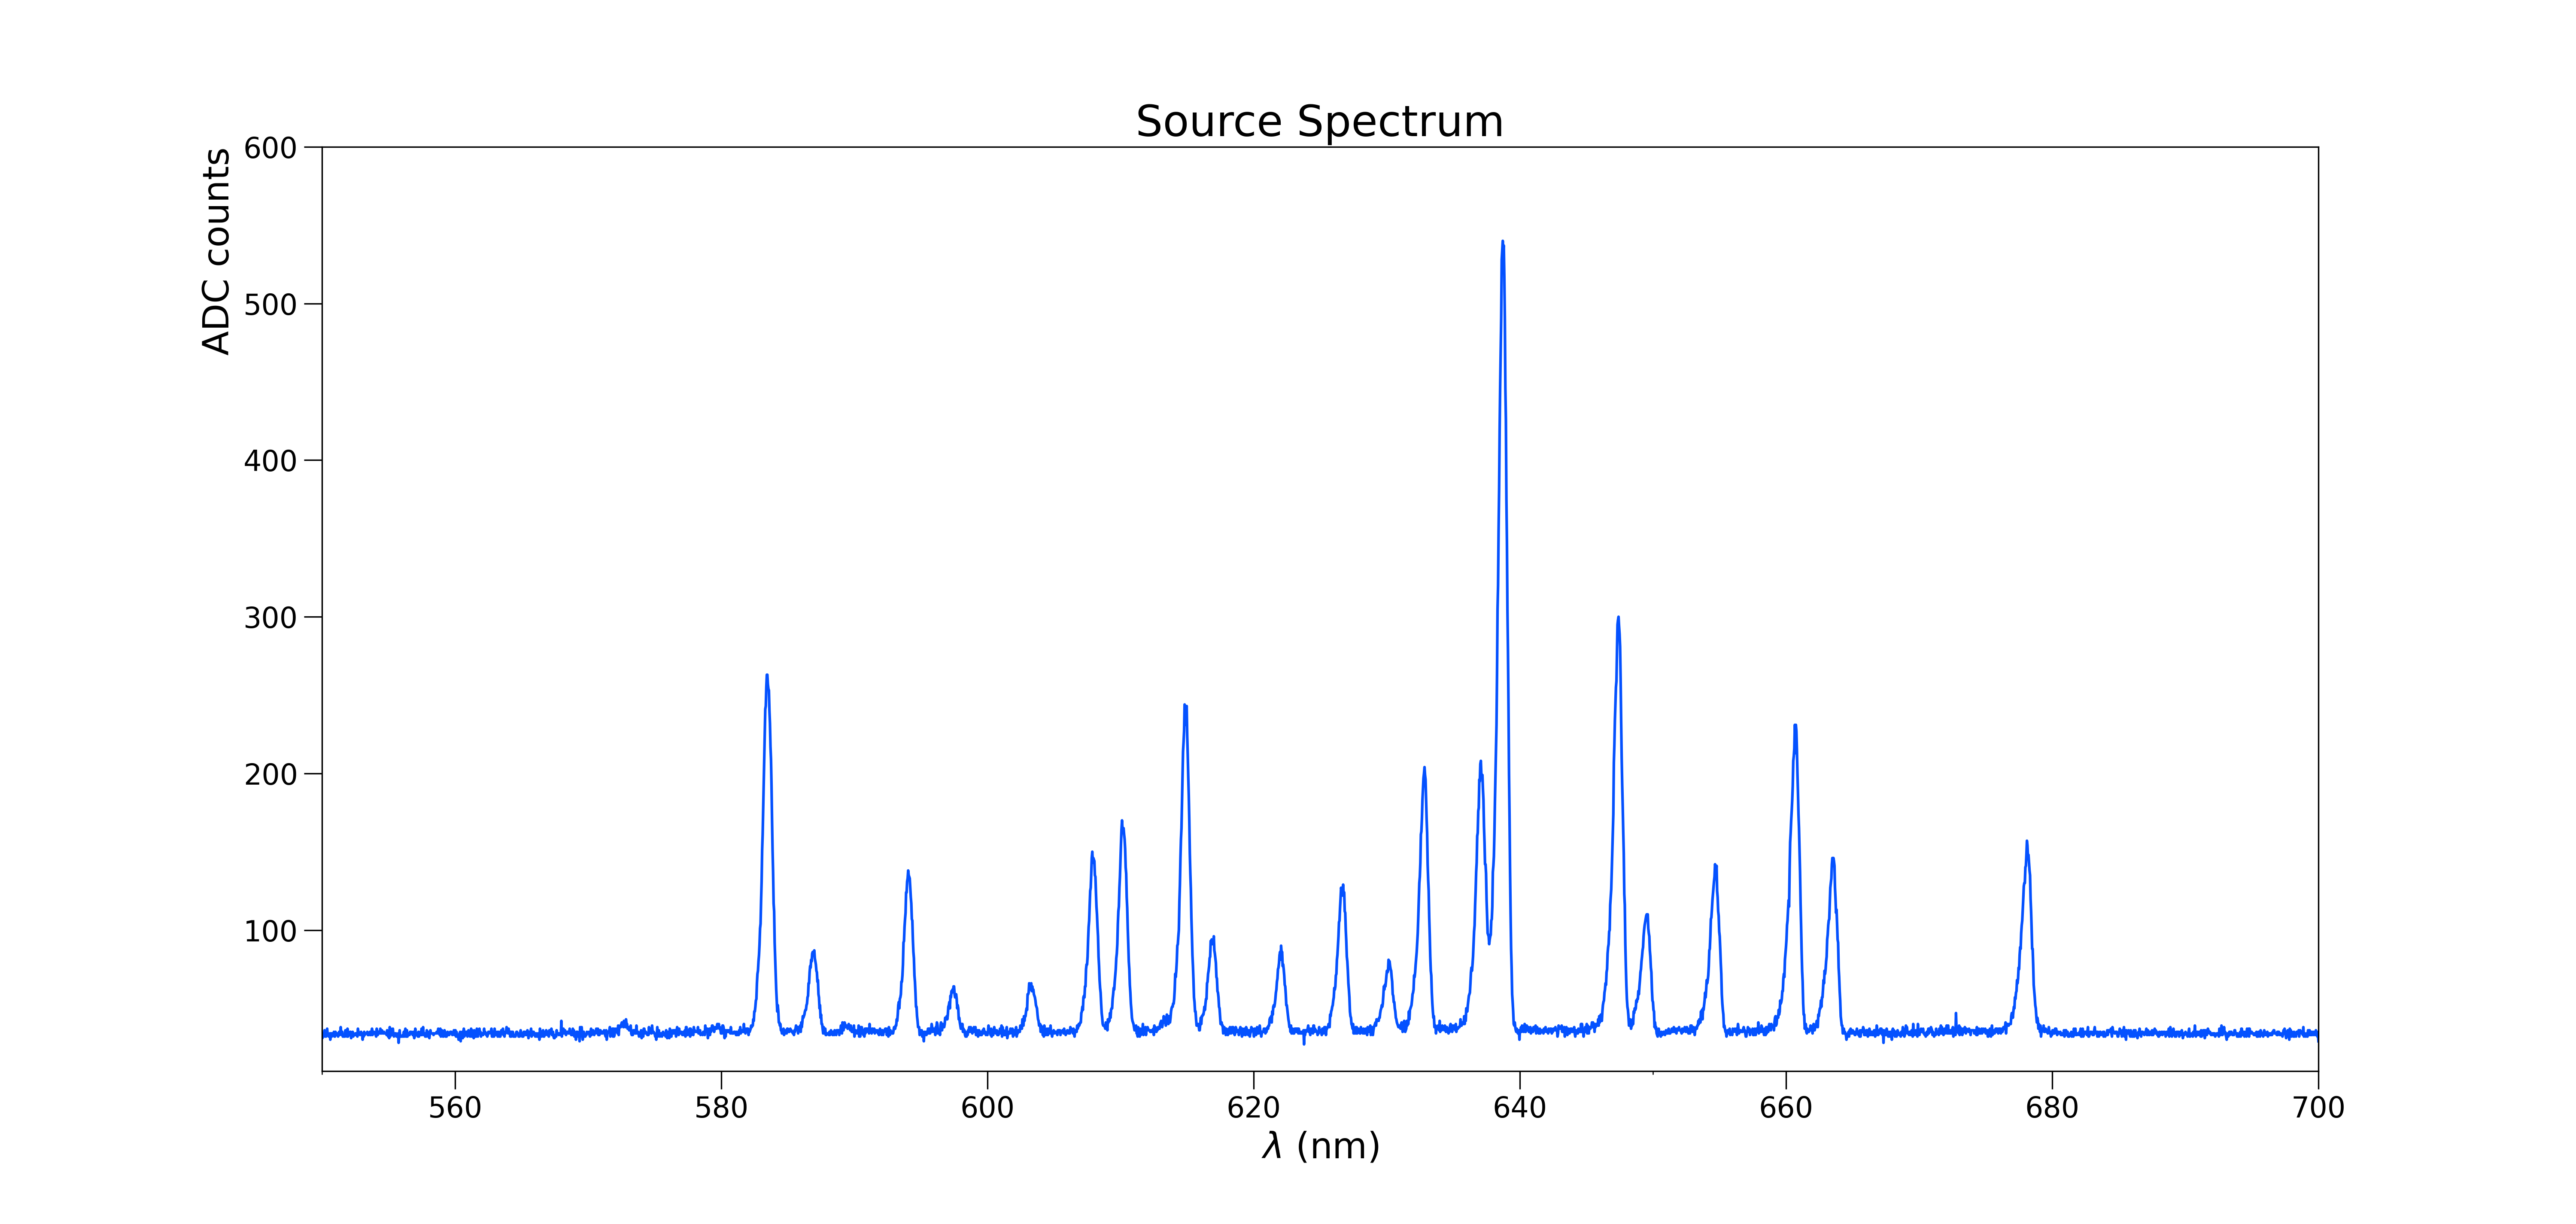
\includegraphics[width=\textwidth]{../Spectrum/SpectrumPlots/spettro1d_Boff.png}
    \caption{Spettro emissivo del Neon con asse orizzontale calibrato}
    \label{i:spettro1d}
\end{figure*}


In \figurename\ref{i:spettro1d} viene rappresentato lo spettro di emissione con l'asse orizzontale calibrato: si
osservano evidenti transizioni nella regione $580-680 \,\si{\nano\metre}$, in particolare la riga più intensa a $640.2
\,\si{\nano\metre}$ e la riga di interesse per l'esperienza a $585.3 \,\si{\nano\metre}$.\\
Si vuole far notare, infine, che in presenza di un campo magnetico esterno lo spettro rimane invariato a meno
dell'intensità della radiazione rivelata, che aumenta significativamente. 




% %%%%%%%%%%%%%%%%%%%%%%%%%%%%%%%%%%%%%%%%%%%%%%%%%%%%%%%%%%%%%%%%%%%%%%
\section{Potere risolvente dell'apparato}\label{s:risolvente}

Il potere risolvente R dell'apparato sperimentale si definisce come

\vspace{-15pt}
\begin{equation}
    R = \frac{\lambda}{\Delta\lambda}
    \label{e:r}
\vspace{-5pt}
\end{equation}

dove, nel caso di interesse, $\lambda = 585.3 \,\si{\nano\metre}$ e $\Delta\lambda$ corrisponde alla larghezza a metà
altezza (in nanometri) dei picchi di interferenza causati dalla lamina di Lummer. Per prima cosa, quindi, sarà
necessario convertire la larghezza dei picchi da pixel del CCD a nanometri: ponendosi nell'approssimazione di luce
radente vale:

\vspace{-10pt}
\begin{equation}
    \Delta\lambda_{\text{r.u.}} \simeq \frac{\lambda^2}{2\text{d}} \approx 0.049\,\si{\nano\metre}
    \label{e:dlambdaru}
\vspace{-5pt}
\end{equation}

Tale quantità corrisponde alla distanza approssimata tra due picchi di interferenza, espressa in nanometri, e dipende
quindi sia dalla lunghezza d'onda della riga $\lambda$ sia dallo spessore della lamina di Lummer d.\\
Conoscendo quindi $\Delta\lambda_{\text{r.u.}}$ è possibile ricavare la larghezza a metà altezza, espressa in nanometri,
dei picchi di interferenza secondo

\vspace{-15pt}
\begin{equation}
    \Delta\lambda = \frac{\Delta\lambda_{\text{r.u.}}}{\Delta x_{\text{r.u.}}} \cdot \Delta x
    \label{e:dlambda}
\vspace{-5pt}
\end{equation}

dove $\Delta x_{\text{r.u.}}$ corrisponde alla distanza tra due picchi espressa in pixel e $\Delta x$ rappresenta la
larghezza a metà altezza dei picchi espressa in pixel.  \\

Si procede quindi restringendo l'intervallo di acquisizione ad un intorno della riga evidenziata in
\autoref{i:spettro1d}: viene quindi ruotato il CCD in posizione verticale e viene inserita la lamina di Lummer. Il tempo
di integrazione scelto per l'acquisizione è di $800\,\si{\milli\second}$. Si sottolinea inoltre che il campo magnetico
rimane spento. \\
Il risultato dell'acquisizione corrisponde allo spettro bidimensionale raffigurato in \autoref{i:spettro2d_Boff} (a
sinistra). A destra invece viene presentata la proiezione sull'asse orizzontale di tale istogramma. In particolare, gli
istogrammi rappresentati in \autoref{i:spettro2d_Boff} sono ottenuti sottraendo il rumore di fondo: nella figura a
sinistra, infatti, si nota chiaramente la presenza della riga di emissione. 

\begin{figure}
    \centering
    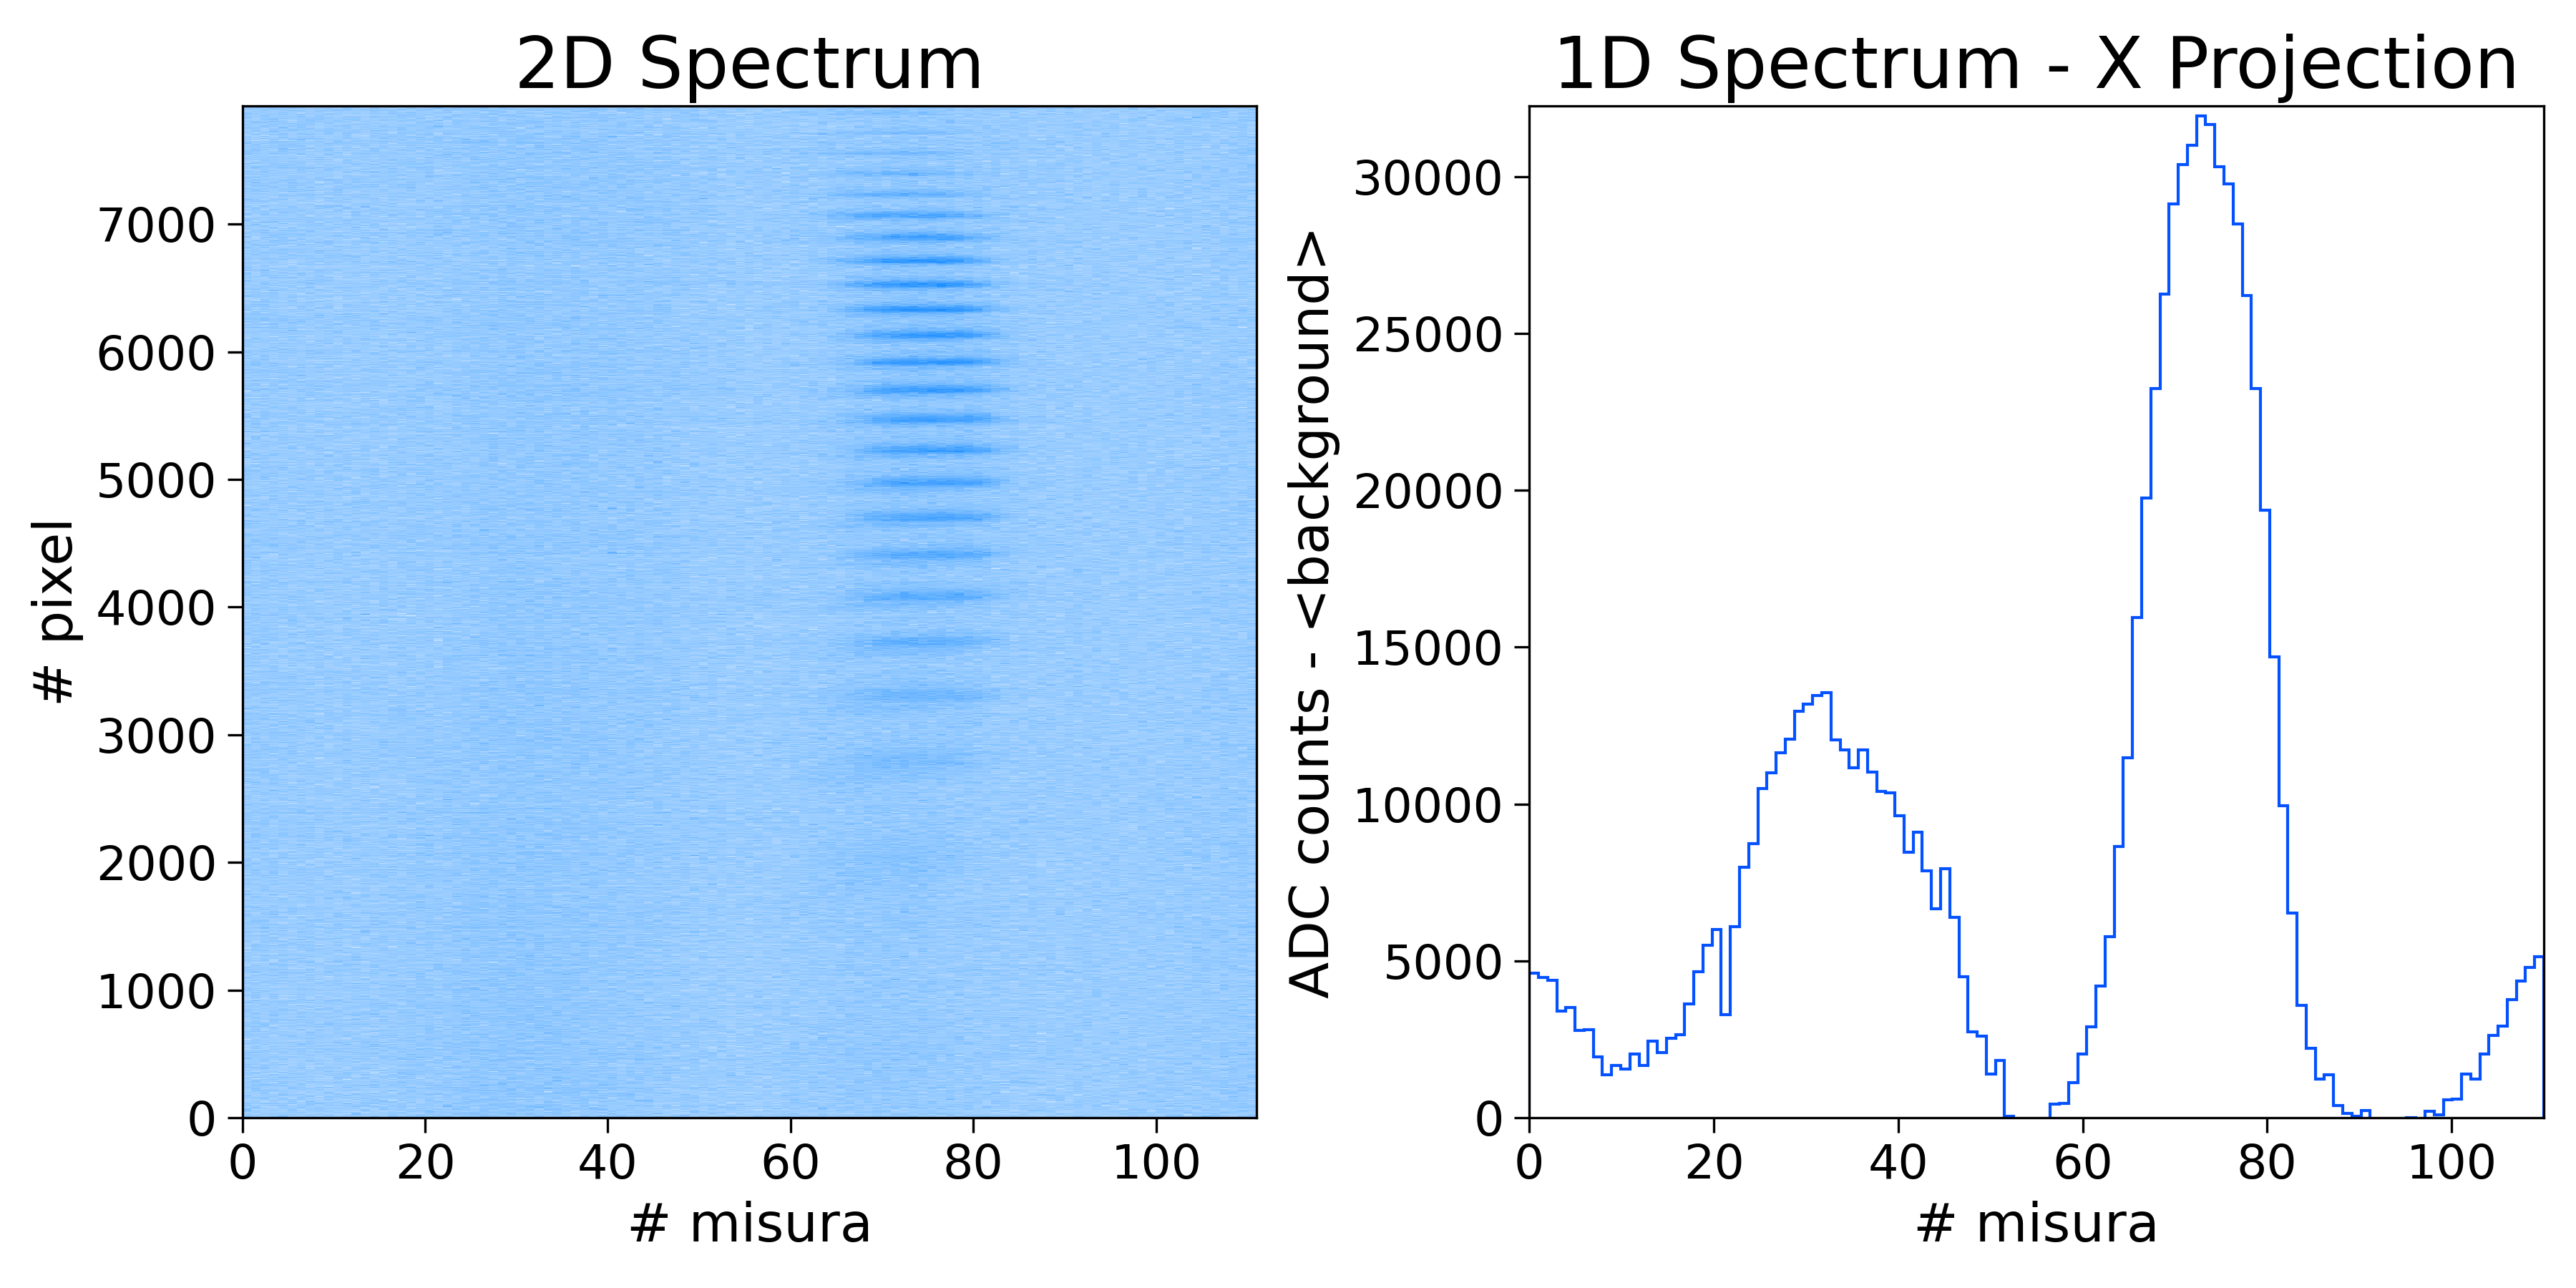
\includegraphics[width=\linewidth]{../Plots/Boff_2d_spectrum.png}
    \caption{Spettro bidimensionale $\text{B}_{\text{off}}$ (a sinistra) e proiezione sull'asse orizzontale (a destra)}
    \label{i:spettro2d_Boff}
    \vspace{-10pt}
\end{figure}

\noindent Per calcolare ora le grandezze di interesse, quali la spaziatura tra picchi e la loro larghezza a metà
altezza, si considera la proiezione dello spettro sull'asse verticale, evidenziando in questo modo le frange di
interferenza causate dalla lamina. Per evitare di ottenere un campione di misure statisticamente dipendenti di $\Delta
x_{\text{r.u.}}$ e $\Delta x$ (e di conseguenza di $\Delta\lambda$ ed R, calcolate a partire dalle prime) si sceglie di
suddividere i picchi di interferenza in triplette contigue. In questo modo, la spaziatura tra i picchi viene calcolata
come media aritmetica della distanza tra i due picchi esterni della tripletta rispetto a quello centrale. Infine, la
larghezza a metà altezza viene misurata unicamente per il picco centrale. Come si può notare in
\autoref{i:spettro2d_Boff_ProjY}, in particolare nel riquadro in alto a sinistra, tutti i picchi vengono fittati da una
funzione gaussiana: la spaziatura tra i picchi viene calcolata utilizzando il centroide delle gaussiane esterne mentre
la FWHM del picco centrale si misura a partire dal valore massimo del fit. Si ottiene, così facendo, un campione di sei
misure di $\Delta x_{\text{r.u.}}$ e $\Delta x$ tra loro statisticamente indipendenti. Si procede dunque al calcolo di
$\Delta\lambda$ secondo \autoref{e:dlambda}, ottenendo infine un campione di poteri risolventi R calcolati seguendo
\autoref{e:r}. Per fornire una stima unica che sia rappresentativa dell'intero apparato si decide di effettuare la media
aritmetica delle misure di R, ottenendo così un potere risolvente pari a 

\begin{figure*}
    \centering
    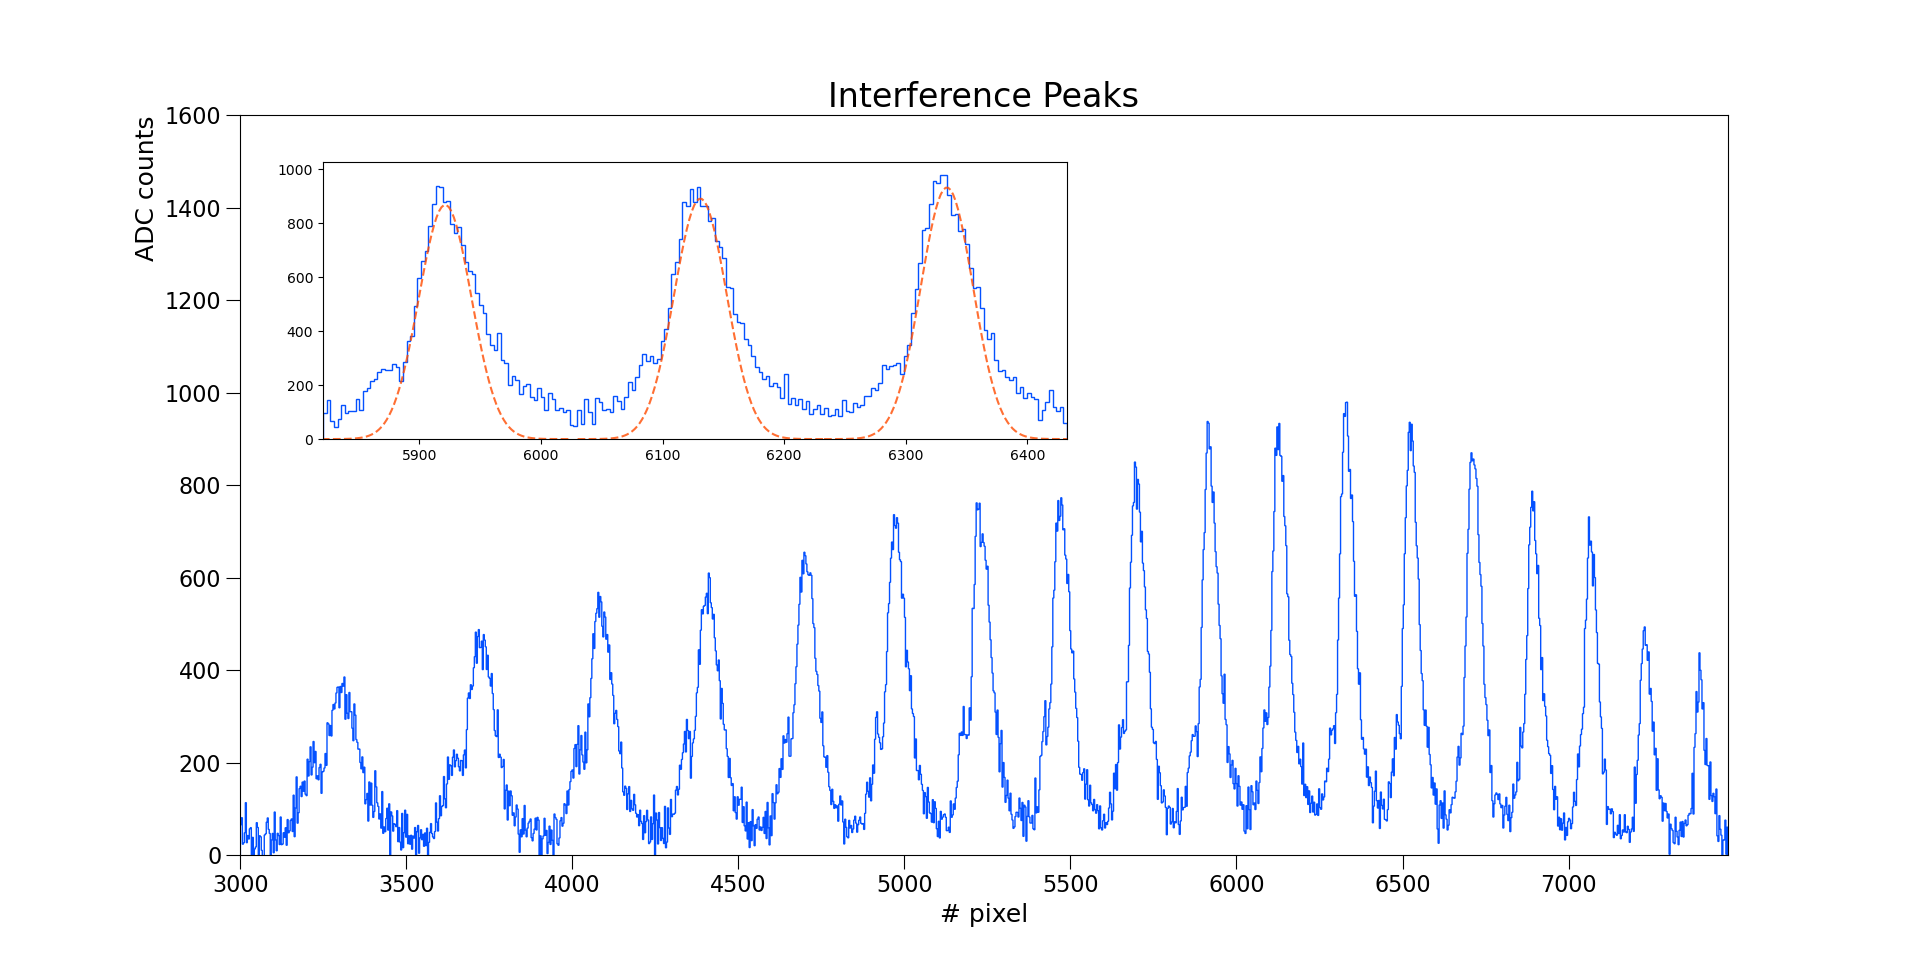
\includegraphics[width=\textwidth]{../Plots/Boff_Y_proj.png}
   \caption{Proiezione sull'asse verticale dello spettro bidimensionale $\text{B}_{\text{off}}$}
    \label{i:spettro2d_Boff_ProjY}
    % \vspace{-10pt}
\end{figure*}

\vspace{-15pt}
\begin{align*}
    \text{R} &= (4.71 \pm 0.10)\cdot 10^4  & \frac{\sigma_{\text{R}}}{\text{R}} &\approx 2\%
    \label{e:R_result}
\vspace{-10pt}
\end{align*}


Risulta quindi che il potere risolvente dell'apparato sia sufficiente da poter rivelare la separazione delle righe
dovuta all'effetto Zeeman. \\
\indent Prima di studiare nel dettaglio l'effetto Zeeman e la sua manifestazione, si preferisce soffermare l'attenzione
ancora brevemente sul grafico in \autoref{i:spettro2d_Boff_ProjY} relativo alle frange di interferenza. Inizialmente, si
vuole far notare che la forma dei picchi è notevolmente variabile in relazione alla posizione di rivelazione sul CCD. Si
è dunque scelto di effettuare fit gaussiani per estrapolare la posizione del centroide e la larghezza per ottenere delle
misure di tali quantità più uniformi tra loro al variare della posizione. Così facendo, infatti, la stima del potere
risolvente risulta essere più precisa di qualche unità percentuale rispetto ad una stima ricavata considerando il
massimo e la larghezza dei picchi stessi (che risultano essere quantità molto variabili e spesso il massimo del picco
non è rappresentativo del centroide della distribuzione). Inoltre, dal grafico si può notare un accentuato effetto di
aberrazione, dovuto alle lenti presenti nell'apparato. Come meglio evidenziato nel grafico in
\autoref{i:spacing_trend_Boff}, questo effetto consiste nella diminuzione progressiva della distanza tra picchi
consecutivi e della loro larghezza. In particolare, la spaziatura tra frange di interferenza (a sinistra) segue
perfettamente un andamento polinomiale di terzo grado (fit in arancione), mentre la loro larghezza (a destra) segue
piuttosto fedelmente un trend lineare. A causa di questo effetto molto influente sulle misure necessarie per il calcolo
del potere risolvente, si è deciso di ricavare un campione di R e successivamente di calcolarne la media, piuttosto che
mediare direttamente i set di dati relativi alle prime. Siccome l'effetto di aberrazione influenza sia la distanza sia
la larghezza in modo sufficientemente simile, la struttura di \autoref{e:dlambda} porta ad una compensazione
soddisfacente di questo fenomeno: il campione di poteri risolventi, infatti, risulta essere composto da misure
casualmente oscillanti e non è stato identificato nessun trend rilevante. Si può quindi concludere che la stima fornita
per R sia robusta e, a meno di approssimazioni, rappresentativa dell'effettivo potere risolvente dell'apparato.

\begin{figure}
    \centering
    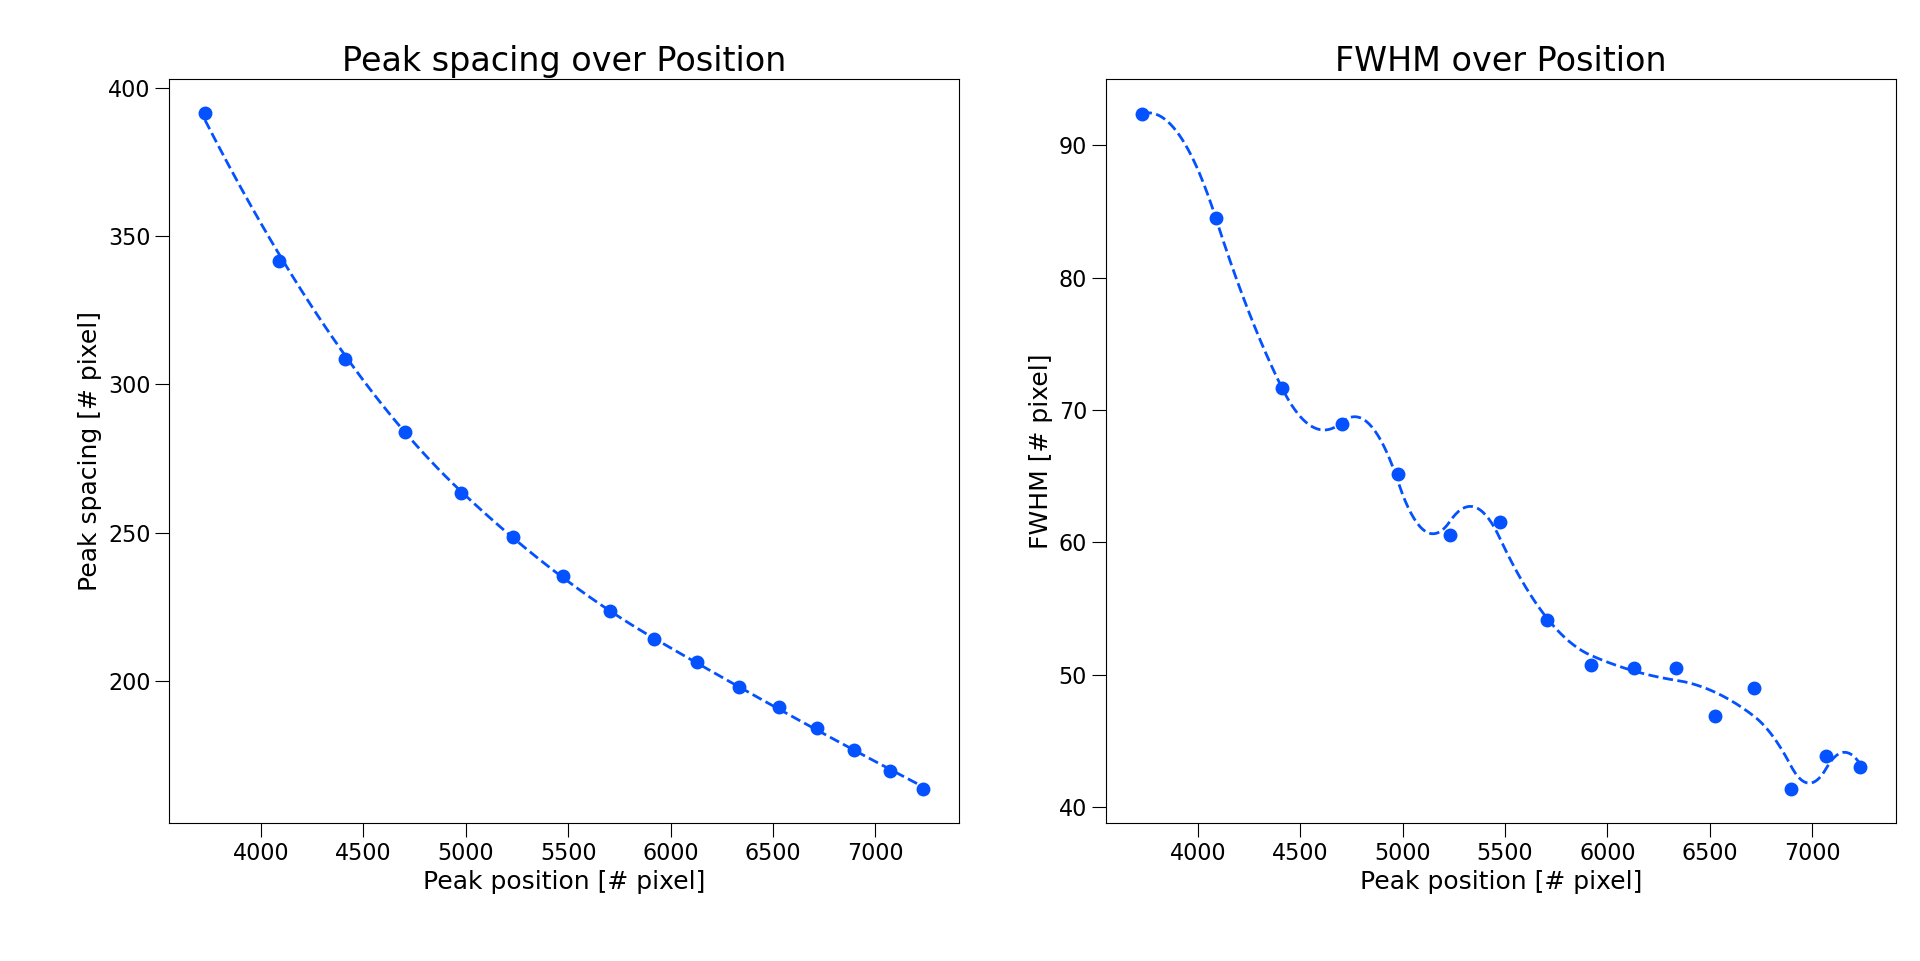
\includegraphics[width=\linewidth]{../Plots/Boff_spacing_trend.png}
    \caption{Andamento della distanza tra i picchi (a sinistra) e della larghezza dei picchi (a destra) in funzione della posizione}
    \label{i:spacing_trend_Boff}
    \vspace{-10pt}
\end{figure}

% QUESTO SERVE PER METTERE DUE FIGURE PICCOLE UNA AFFIANCO ALL'ALTRA
% \begin{figure*}[htp]
%     \centering
%     \subfigure[Spettro bidimensionale $\text{B}_{\text{off}}$]{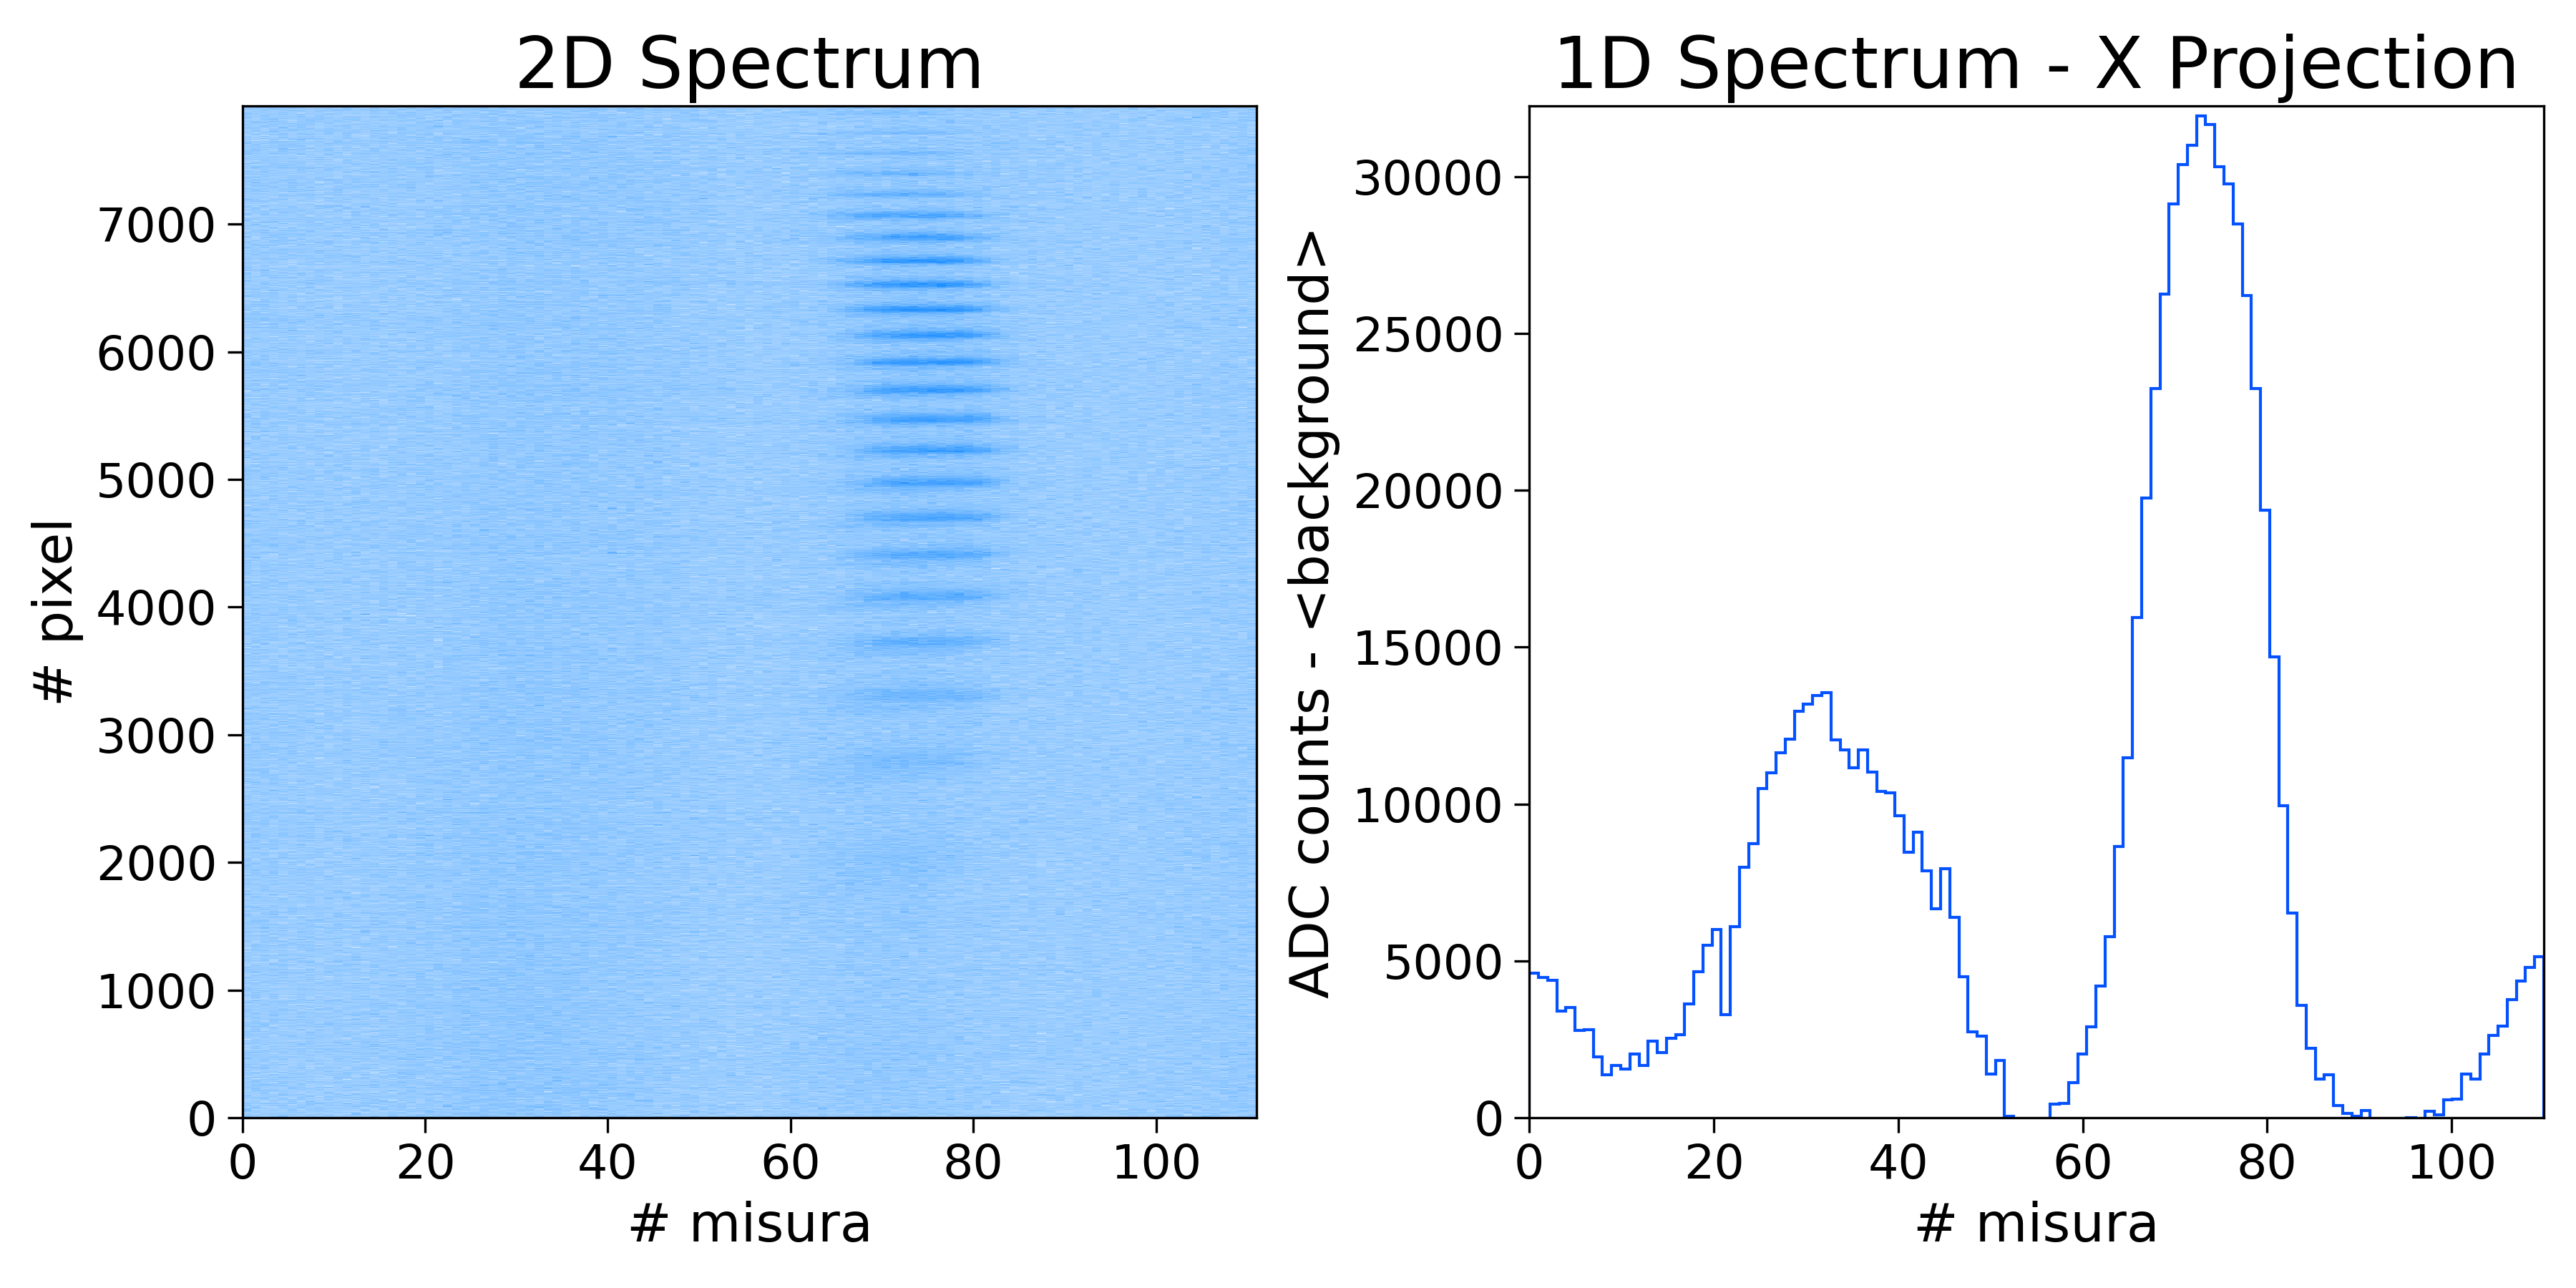
\includegraphics[width=0.5\textwidth]{../Plots/Boff_2d_spectrum.png}}\label{i:spettro2d_Boff}\hfill
%     \subfigure[Spacing trend]{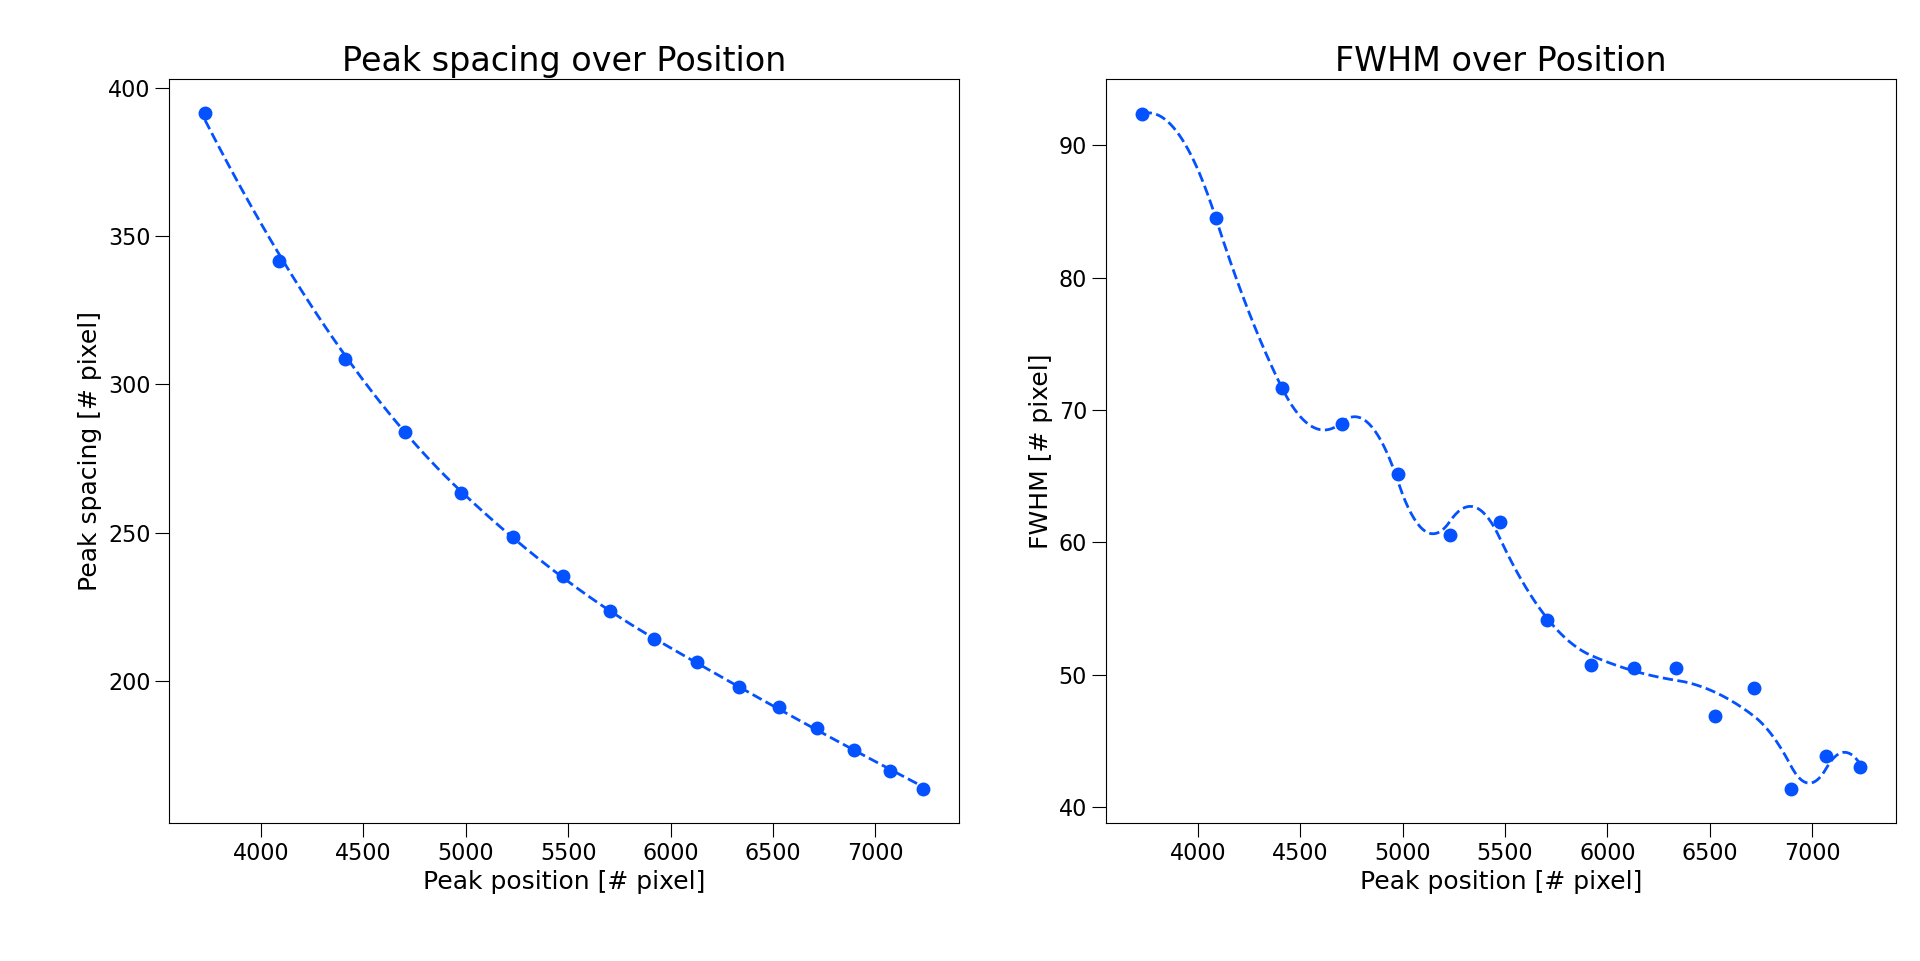
\includegraphics[width=0.5\textwidth]{../Plots/Boff_spacing_trend.png}}\label{i:spacing_trend_Boff}
%   \end{figure*}



% %%%%%%%%%%%%%%%%%%%%%%%%%%%%%%%%%%%%%%%%%%%%%%%%%%%%%%%%%%%%%%%%%%%%%%
\section{Fattore di Landè}\label{s:lande}

% \begin{itemize}
%     \item Lo calcoliamo con Bon lungo la direzione della radiazione (parlare dello splitting di Zeeman)
%     \item Formule (range utile + conversione energia + fattore di Landè)
%     \item Procedura di analisi (niente fit perchè non vengono)
%     \item Plot con tutti i picchi + finestrella con lo zoom su una tripletta 
%     \item Controllare che lo splitting Zeeman non subisca aberrazione pesante
% \end{itemize}

Disponendo di un apparato strumentale con sufficiente potere risolutivo, ci si propone ora di studiare la manifestazione
dell'effetto Zeeman, ovvero la separazione dei livelli energetici e, di conseguenza, delle righe spettrali. Come
verifica della corretta osservazione del fenomeno, si vuole misurare il fattore di Landè $\text{g}_{\text{J}}$ che, 
data la transizione $^1\text{S}_0 \rightarrow ^1\text{P}_1$ in studio, deve risultare pari ad uno.

Il fattore di Landè si ricava dalla relazione

\vspace{-15pt}
\begin{equation}
    \Delta \text{E}_{\text{zee}} = - \text{g}_{\text{J}} \mu_{\text{B}} \text{m}_{\text{j}} \text{B} 
    \label{e:gL}
\vspace{-5pt}
\end{equation}

dove $\mu_{\text{B}}$ è il magnetone di Bohr e $\Delta \text{E}_{\text{zee}}$ corrisponde alla separazione dei livelli
energetici dovuta al campo magnetico esterno B. Configurando il campo magnetico parallelamente alla direzione di
propagazione i termini polarizzati circolarmente corrispondenti a $\Delta \text{m} = \pm 1$ hanno intensità maggiore dei
termini corrispondenti a $\Delta \text{m} = 0$. Ne consegue quindi che la transizione centrale risulta soppressa e si
riescono ad osservare solo le due laterali, separate da $\delta\lambda = 2 \Delta\lambda_{\text{zee}}$, dove
$\Delta\lambda_{\text{zee}}$ rappresenta lo splitting Zeeman. 

\begin{figure*}
    \centering
    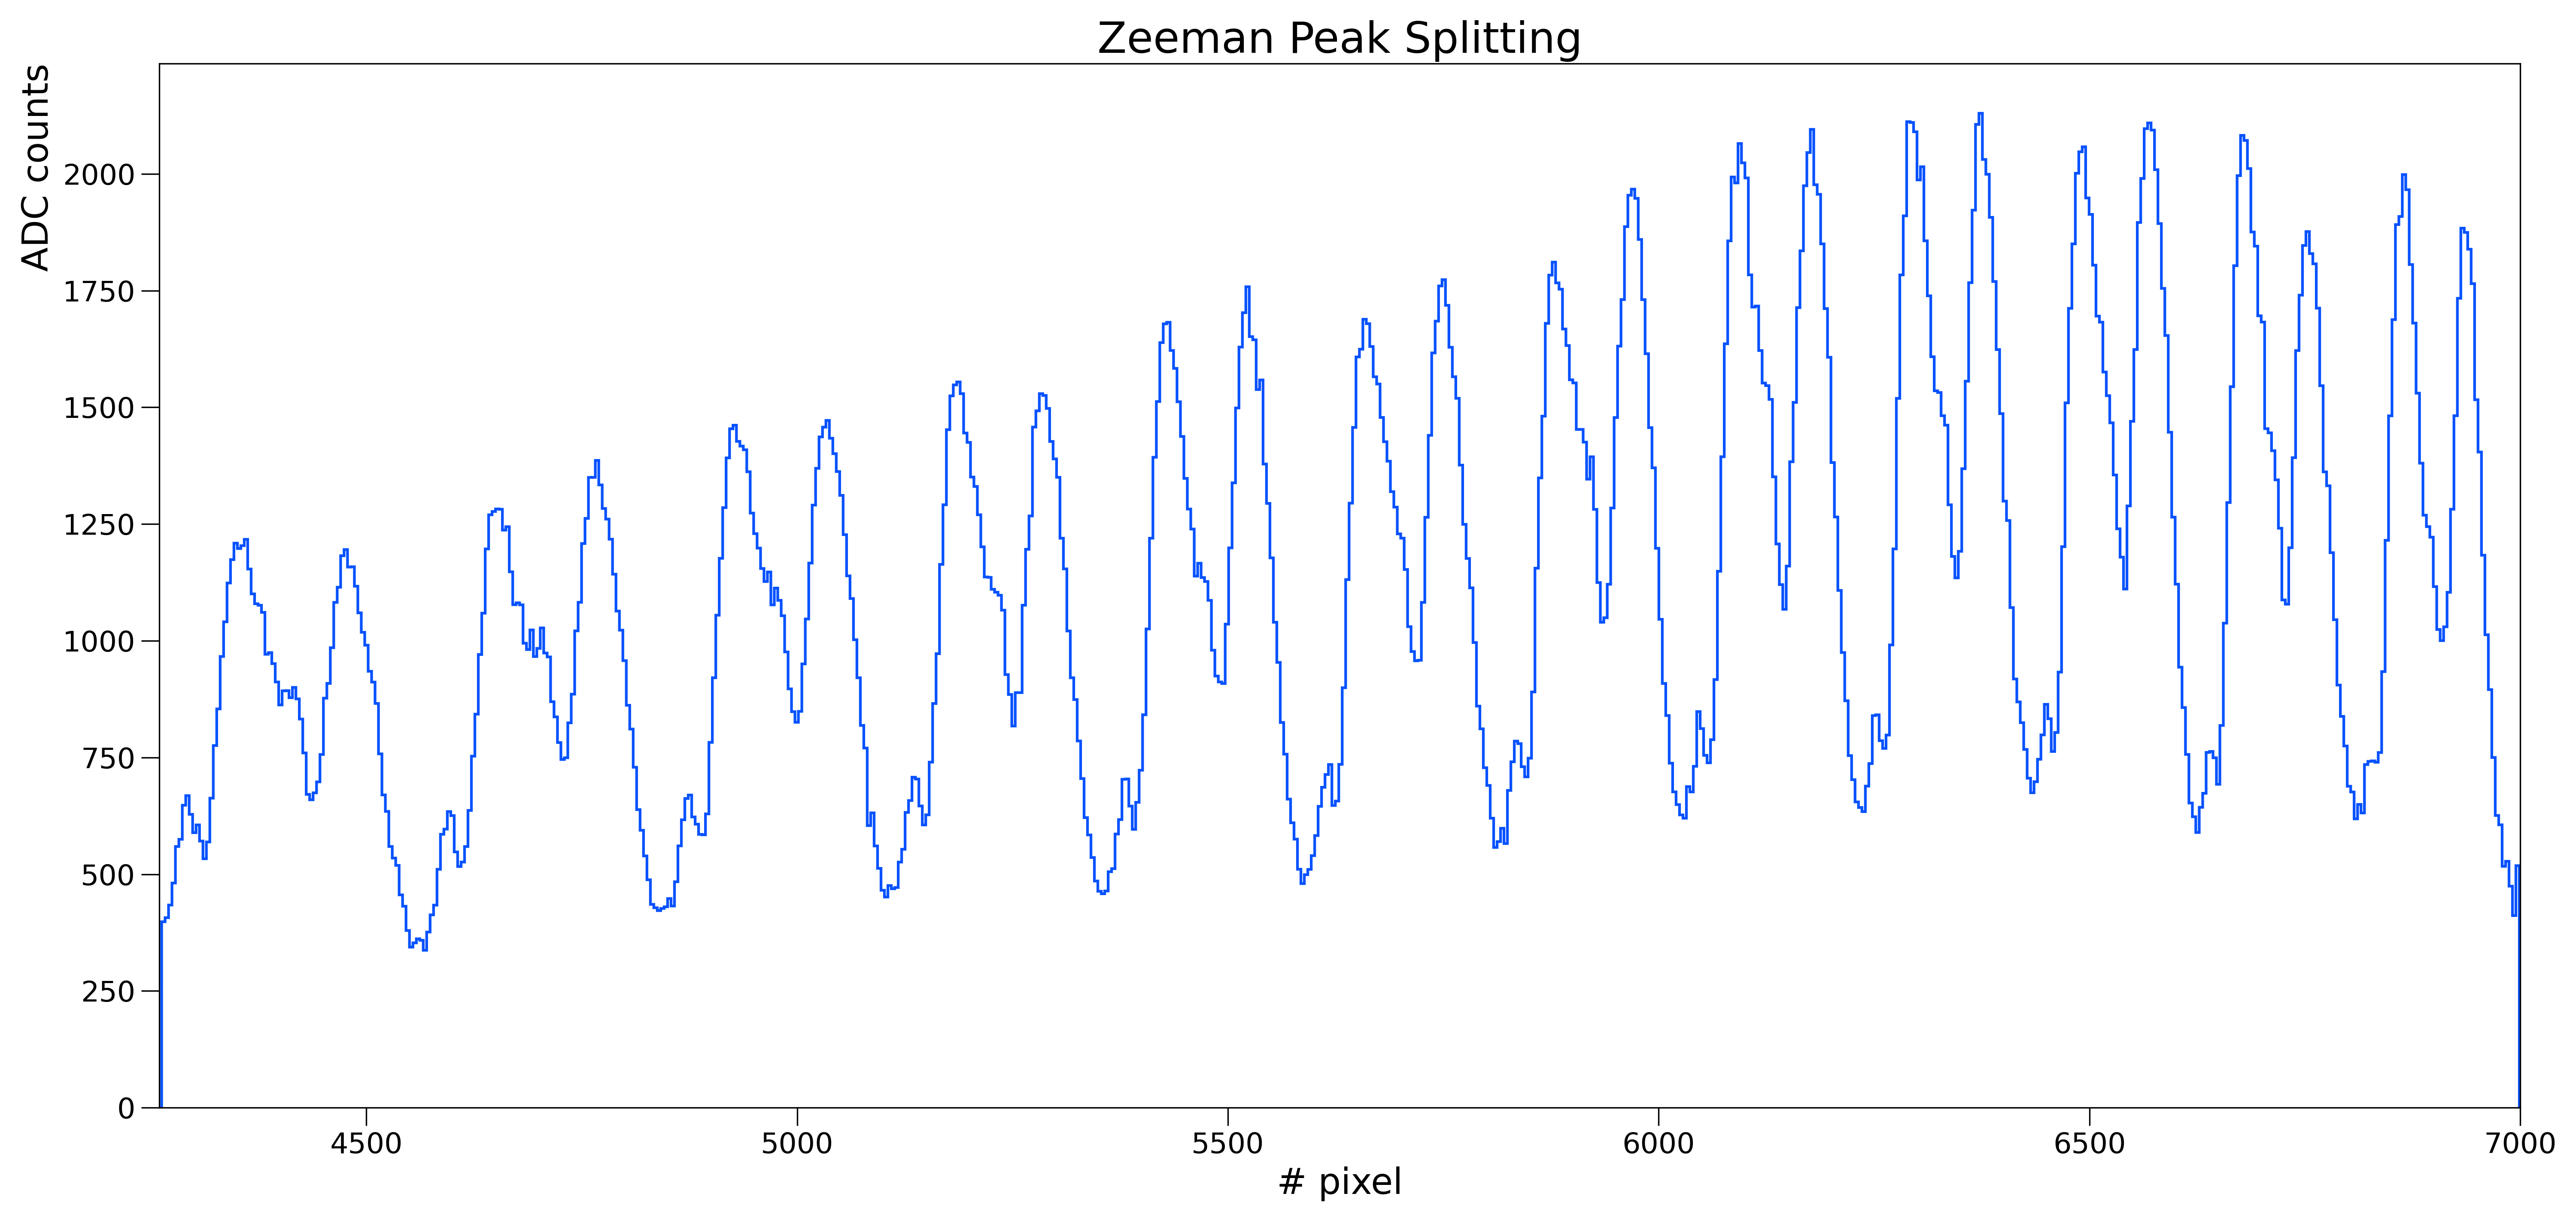
\includegraphics[width=\textwidth]{../Plots/Bon_Y_proj.png}
    \caption{Proiezione sull'asse verticale $\text{B}_{on}$}
    \label{i:spettro2d_Bon_ProjY}
\end{figure*}

\noindent Tale separazione in lunghezza d'onda, che è la quantità misurabile con lo spettrometro a disposizione, è legata alla
separazione energetica dalla relazione

\vspace{-15pt}
\begin{equation}
    \Delta \text{E}_{\text{zee}} = \frac{\text{hc}}{\lambda^2} \cdot \Delta\lambda_{\text{zee}}
    \label{e:dEzee}
\vspace{-5pt}
\end{equation}

Si procede dunque impostando il campo magnetico ad un'intensità di $\text{B} = 0.522 \pm 0.005 \,\si{\tesla}$ in
direzione parallela al fascio. Successivamente, in analogia con quanto riportato in \autoref{s:risolvente}, viene
identificata la riga a $\lambda = 585.3 \,\si{\nano\metre}$ e viene acquisito uno spettro bidimensionale in uno stretto
intorno del picco di interesse usando come tempo di integrazione $800\,\si{\milli\second}$. Tale spettro, assieme alla
proiezione sull'asse orizzontale, è raffigurato in \autoref{i:spettro2d_Bon}. \\
Per osservare lo splitting causato dalla presenza del campo magnetico si considera dunque la proiezione dello spettro
sull'asse verticale, evidenziando così le frange di interferenza. Come si può notare immediatamente osservando il
grafico in \autoref{i:spettro2d_Bon_ProjY}, a differenza di quanto riportato in \autoref{i:spettro2d_Boff_ProjY} i
picchi ora presentano una evidente separazione, pressochè simmetrica, a partire da circa metà altezza. 

\begin{figure}
    \centering
    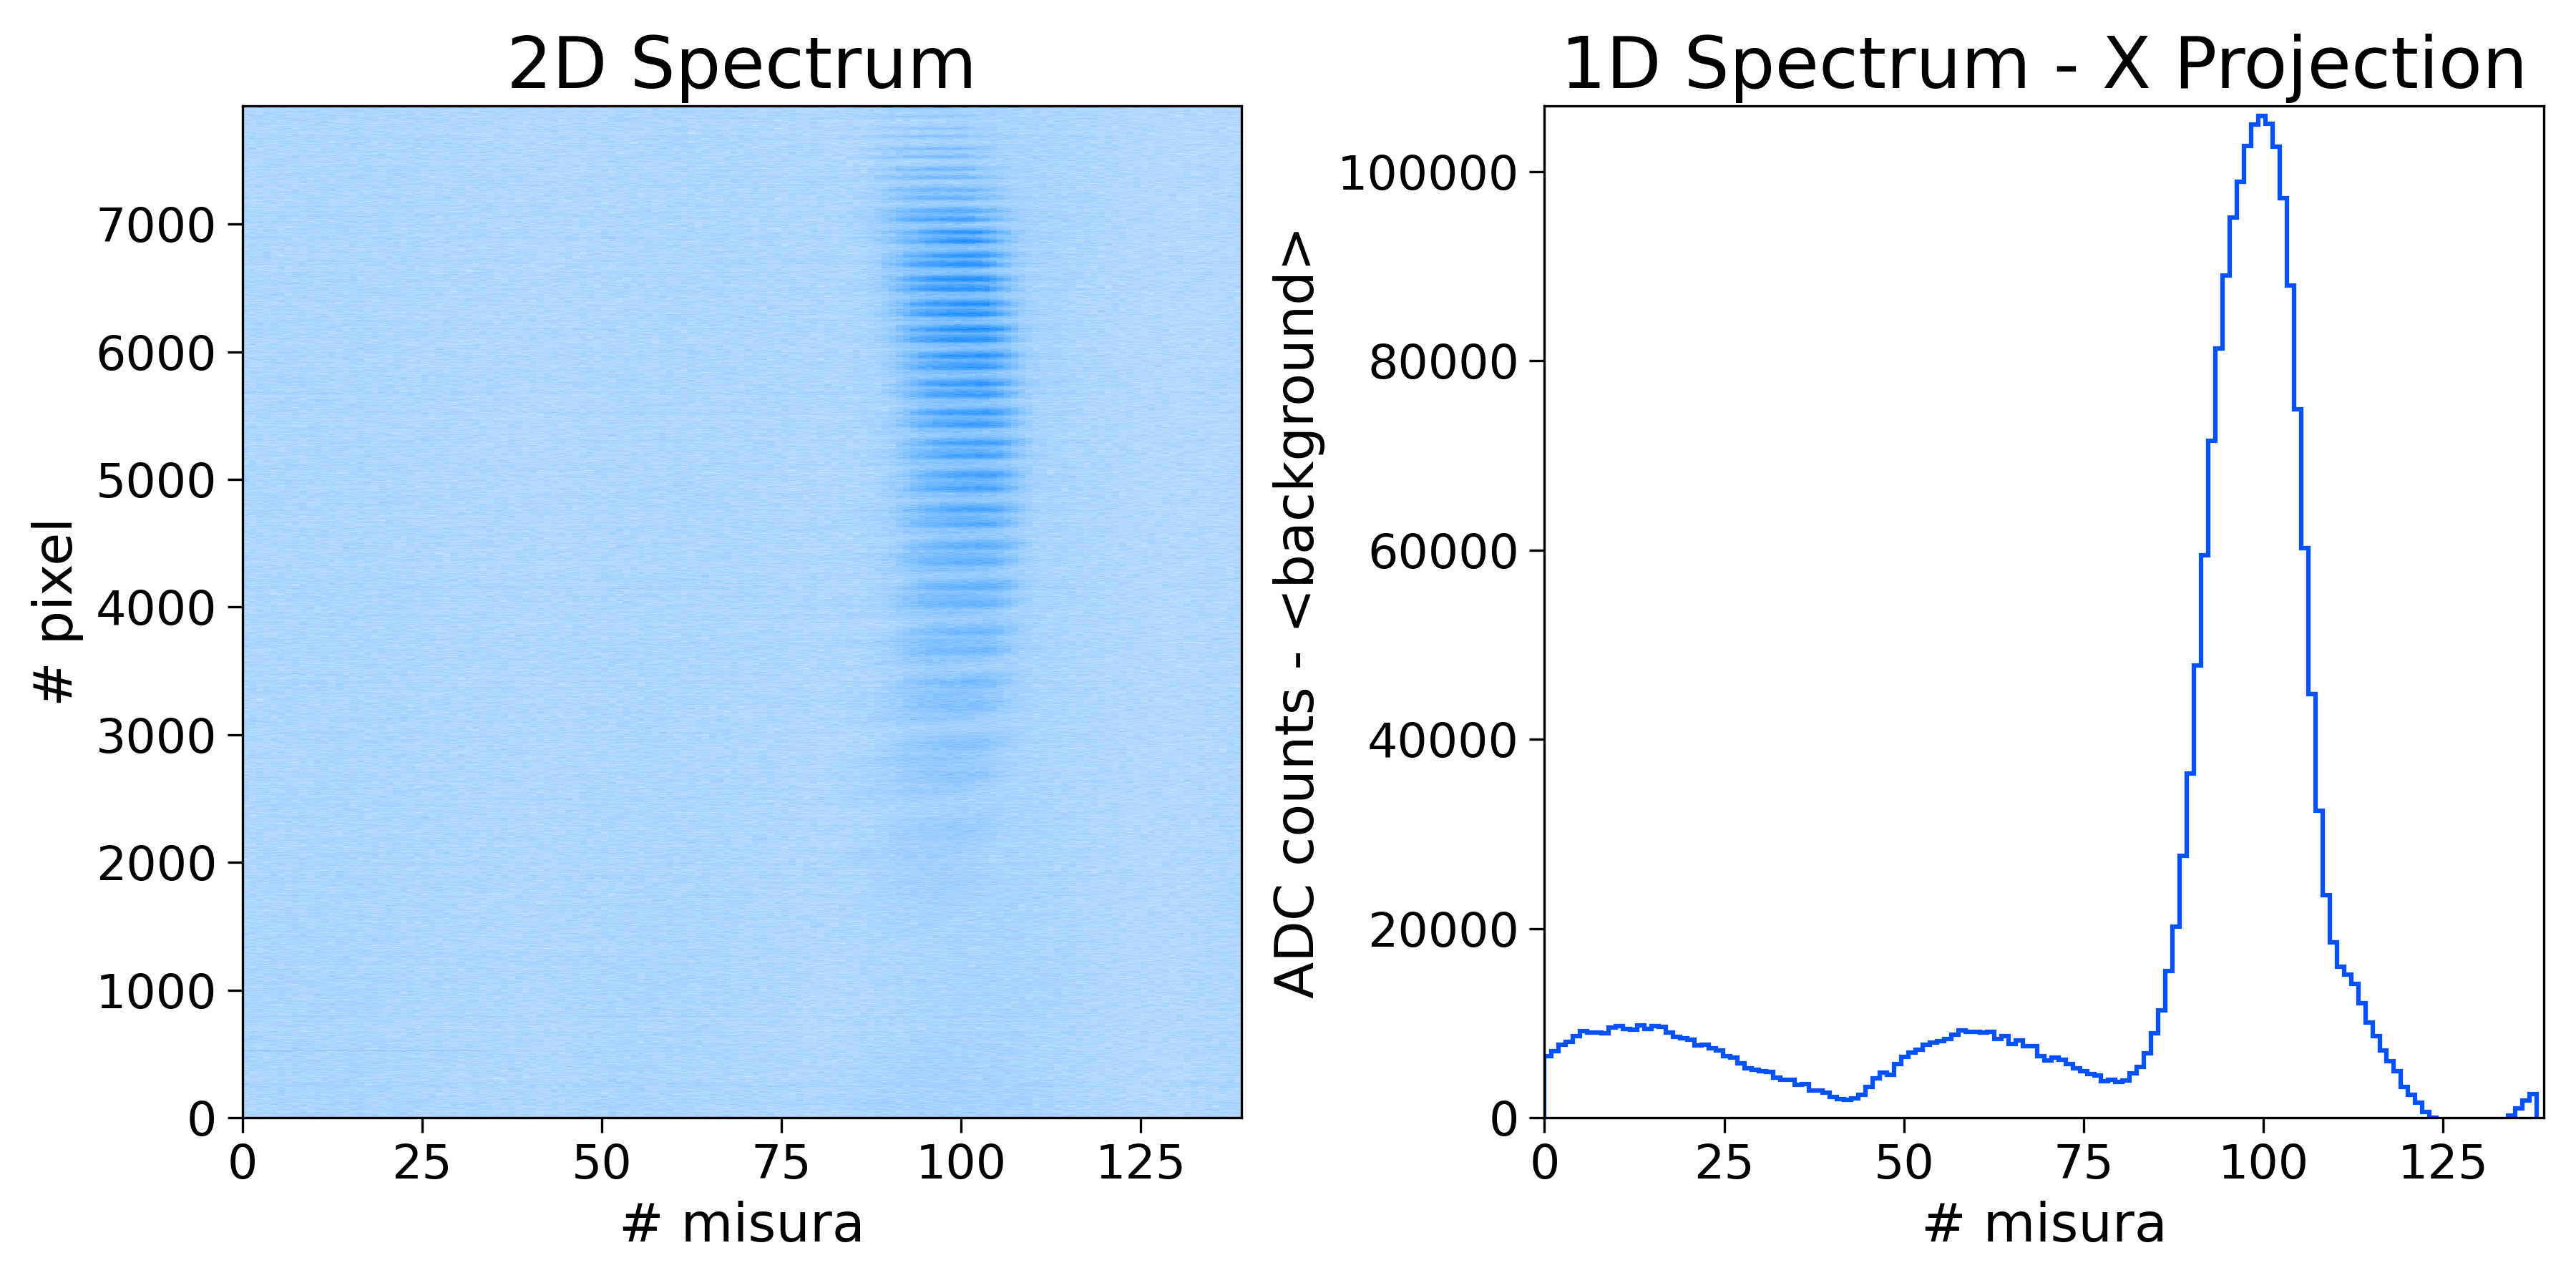
\includegraphics[width=\linewidth]{../Plots/Bon_2d_spectrum.png}
    \caption{Spettro bidimensionale $\text{B}_{\text{on}}$ (a sinistra) e proiezione sull'asse orizzontale (a destra)}
    \label{i:spettro2d_Bon}
\end{figure}

\noindent Volendo essere più precisi nello studio, risulta necessario misurare la separazione dei picchi causata dal
campo magnetico. Successivamente, tale distanza (misurata in pixel) viene convertita in nanometri sfruttando la
relazione in \autoref{e:dlambda}: $\Delta\lambda_{\text{r.u.}}$ rimane invariata rispetto alla sezione precedente,
$\Delta x_{\text{r.u.}}$ rappresenta nuovamente la distanza tra due frange di interferenza ma necessita di essere
ricalcolata con maggior accortezza, mentre $\Delta x$ ora rappresenza invece la separazione dei picchi espressa in
pixel. In questo modo, sfruttando \autoref{e:dlambda}, si ricava una stima per $\delta\lambda = 2
\Delta\lambda_{\text{zee}}$. In analogia con quanto riportato in \autoref{s:risolvente}, si suddividono le frange di
interferenza in triplette contigue. Contrariamente a quanto effettuato in precedenza, invece, non si è in grado di
fittare i picchi separati in quanto non presentano una sufficiente forma gaussiana. Per il calcolo delle quantità
necessarie si è dunque costretti ad utilizzare i dati stessi, con la consapevolezza che questo tipo di approccio avrà un
impatto non indifferente sulla precisione delle stime successive.

Per calcolare $\Delta x_{\text{r.u.}}$, la strategia adottata è la seguente. Inizialmente, viene identificata
(approssimativamente) la posizione centrale dei picchi separati dall'effetto del campo effettuando una media delle
posizioni dei due massimi splittati. Successivamente, si calcolano la distanza tra il primo picco e quello centrale e
tra quest'ultimo ed il terzo picco della tripletta. Quindi, $\Delta x_{\text{r.u.}}$ viene stimata come media di queste
due distanze. Per quanto riguarda $\Delta x$, invece, si considera la distanza di separazione dei picchi della frangia
centrale. \\
Si ottiene quindi un campione di misure di $\Delta\lambda_{\text{zee}}$ (la cui media risulta essere
$\langle\Delta\lambda_{\text{zee}}\rangle = 0.00863 \pm 0.00012 \,\si{\nano\metre}$, in accordo con le previsioni del
fenomeno): utilizzando la relazione in \autoref{e:dEzee} viene quindi calcolato un campione relativo alla separazione
energetica $\Delta \text{E}_{\text{zee}}$. Successivamente, esplicitando il fattore di Landè da \autoref{e:gL}, si
ottiene un campione di $\text{g}_{\text{J}}$: a queste misure viene associata un'incertezza data dalla propagazione

\vspace{-15pt}
\begin{equation}
    \sigma_{\text{g}_{\text{J}}} = \text{g}_{\text{J}} \, 
    \sqrt{ 
        \left(\frac{\sigma_{\Delta \text{E}_{\text{zee}}}}{\Delta \text{E}_{\text{zee}}}\right)^2 + 
        \left(\frac{\sigma_{\text{B}}}{\text{B}}\right)^2
        }
    \vspace{-5pt}
\end{equation}

\noindent dove $\sigma_{\Delta \text{E}_{\text{zee}}}$ è lo scarto quadratico medio del campione di misure relative alla
separazione energetia, mentre $\sigma_{\text{B}}$ è l'$1\%$ del valore del campo magnetico esterno. 

Infine, la stima del fattore di Landè viene trovata effettuando una media pesata tra le misure del campione, ottenendo
così 

\vspace{-15pt}
\begin{align*}
    \text{g}_{\text{J}} &= 1.033 \pm 0.014 & \frac{\sigma_{\text{g}_{\text{J}}}}{\text{g}_{\text{J}}} &\approx 1.4\%
    \vspace{-5pt}
\end{align*}

Il fattore così misurato risulta essere in soddisfacente accordo con le previsioni teoriche, presentando una
compatibilità pari a $2.4$ con tale valore di aspettazione. Ovviamente, a causa dell'approccio, piuttosto
approssimativo, utilizzato per analizzare i dati, la non ottima compatibilità con le aspettative teoriche è stata
prevista: volendo indagare più a fondo si propone un breve studio sull'andamento dello splitting Zeeman delle frange in
funzione della posizione. Come si può notare in \autoref{i:spacing_trend_Bon}, in particolare osservando il grafico a
sinistra, l'effetto di aberrazione, oltre ad influire sulla distanza tra picchi e sulla loro larghezza come evidenziato
in \autoref{s:risolvente}, modifica la speparazione delle frange al variare della posizione. L'andamento di tale
separazione, infatti, segue un trend piuttosto lineare che ricorda in particolar modo l'andamento della larghezza dei
picchi riportato in \autoref{i:spacing_trend_Boff}.


\begin{figure}
    \centering
    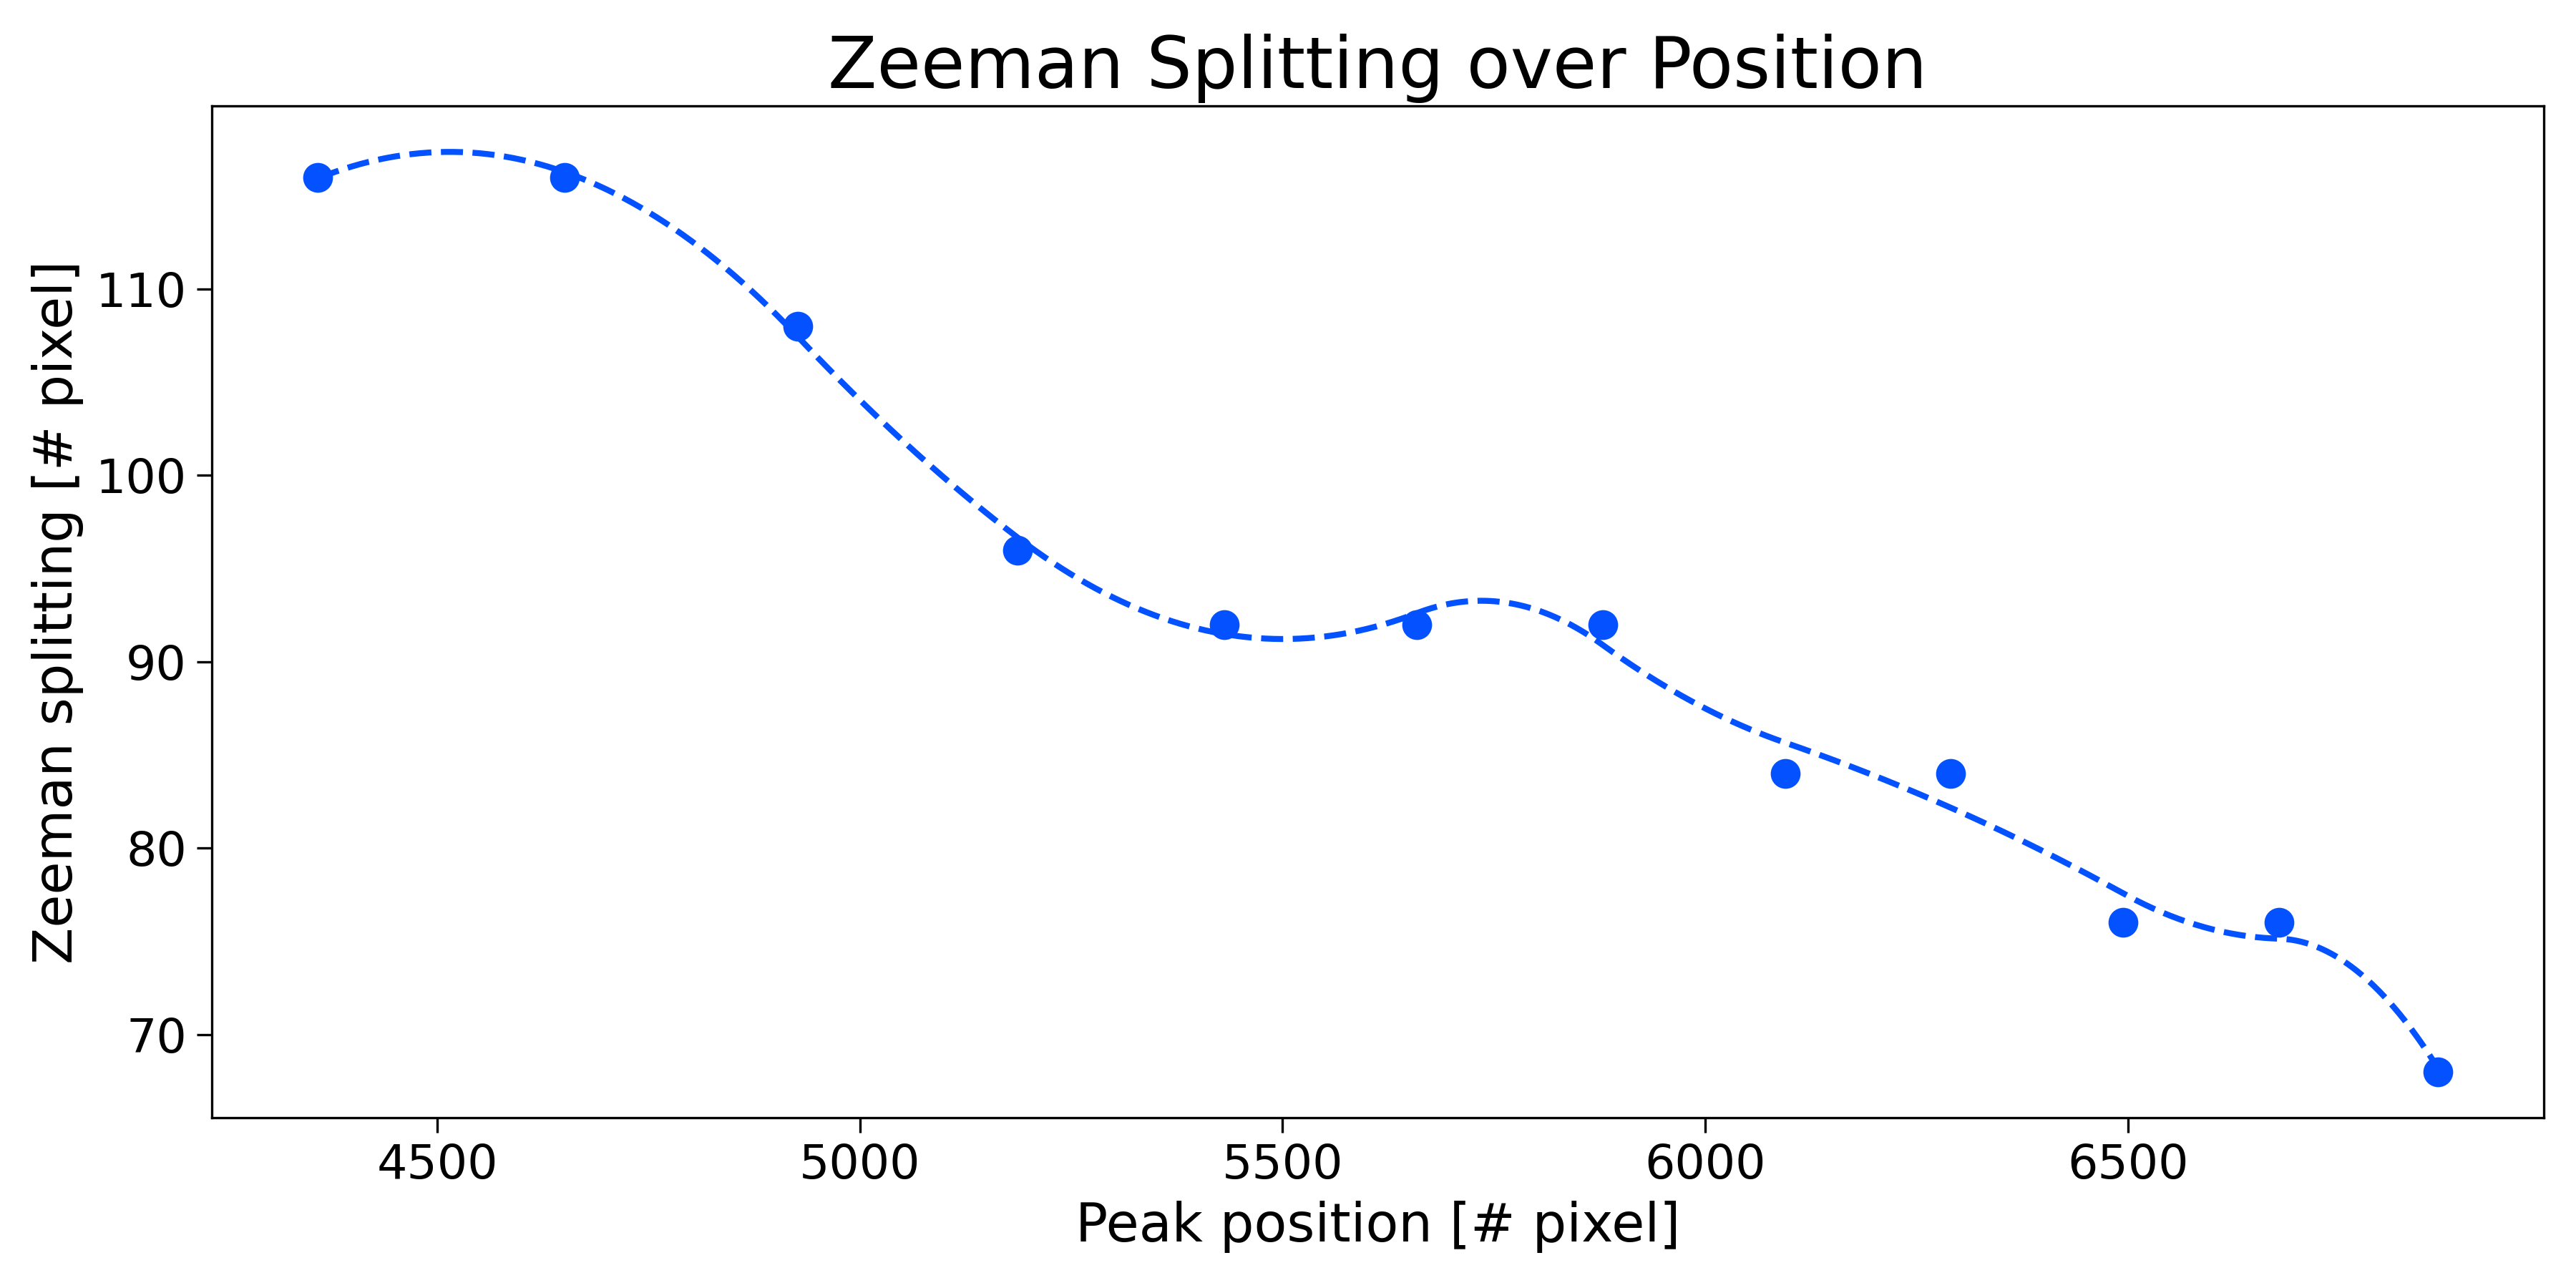
\includegraphics[width=\linewidth]{../Plots/Bon_zeeman_trend.png}
    \caption{Andamento della separazione Zeeman tra picchi (a sinistra) e del rapporto tra distanza tra picchi e separazione Zeeman (a destra) in funzione della posizione}
    \label{i:spacing_trend_Bon}
    \vspace{-10pt}
\end{figure}


% \begin{figure}
%     \centering
%     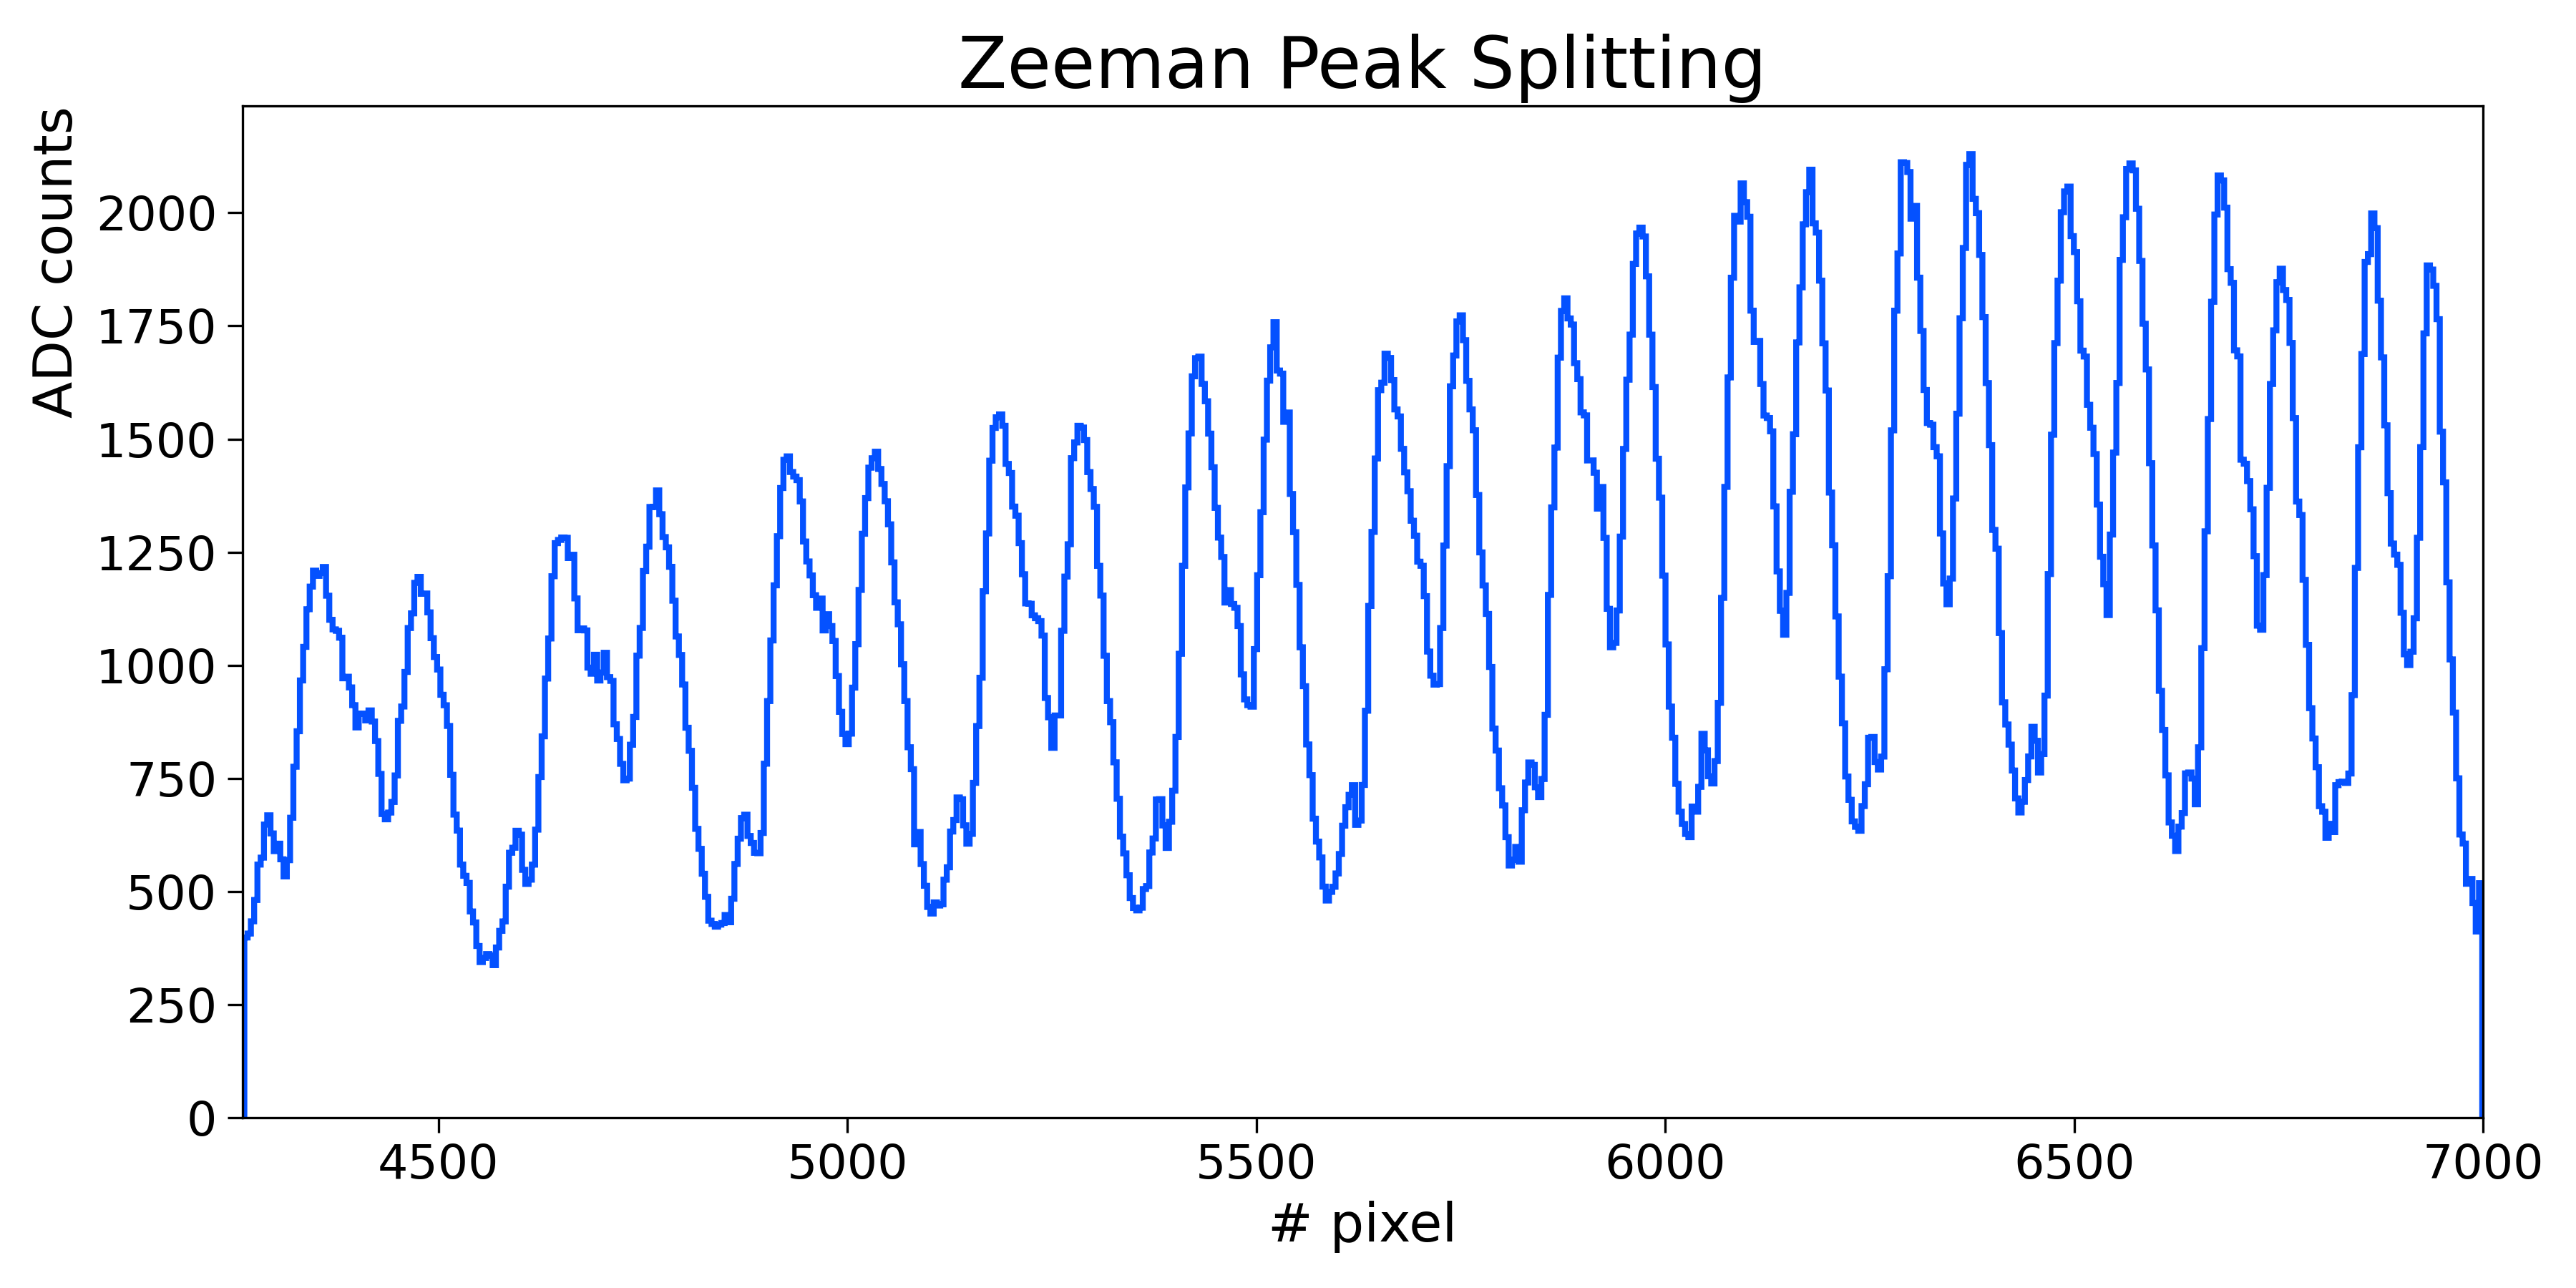
\includegraphics[width=\linewidth]{../Plots/Bon_Y_proj2_small.png}
%     \caption{Proiezione sull'asse verticale $\text{B}_{on}$}
%     \label{i:spettro2d_Bon_ProjY}
% \end{figure}







\cleardoublepage
% %%%%%%%%%%%%%%%%%%%%%%%%%%%%%%%%%%%%%%%%%%%%%%%%%%%%%%%%%%%%%%%%%%%%%%
\section{Campo magnetico ortogonale alla radiazione}\label{s:ortogonale}

\begin{figure*}
    \centering
    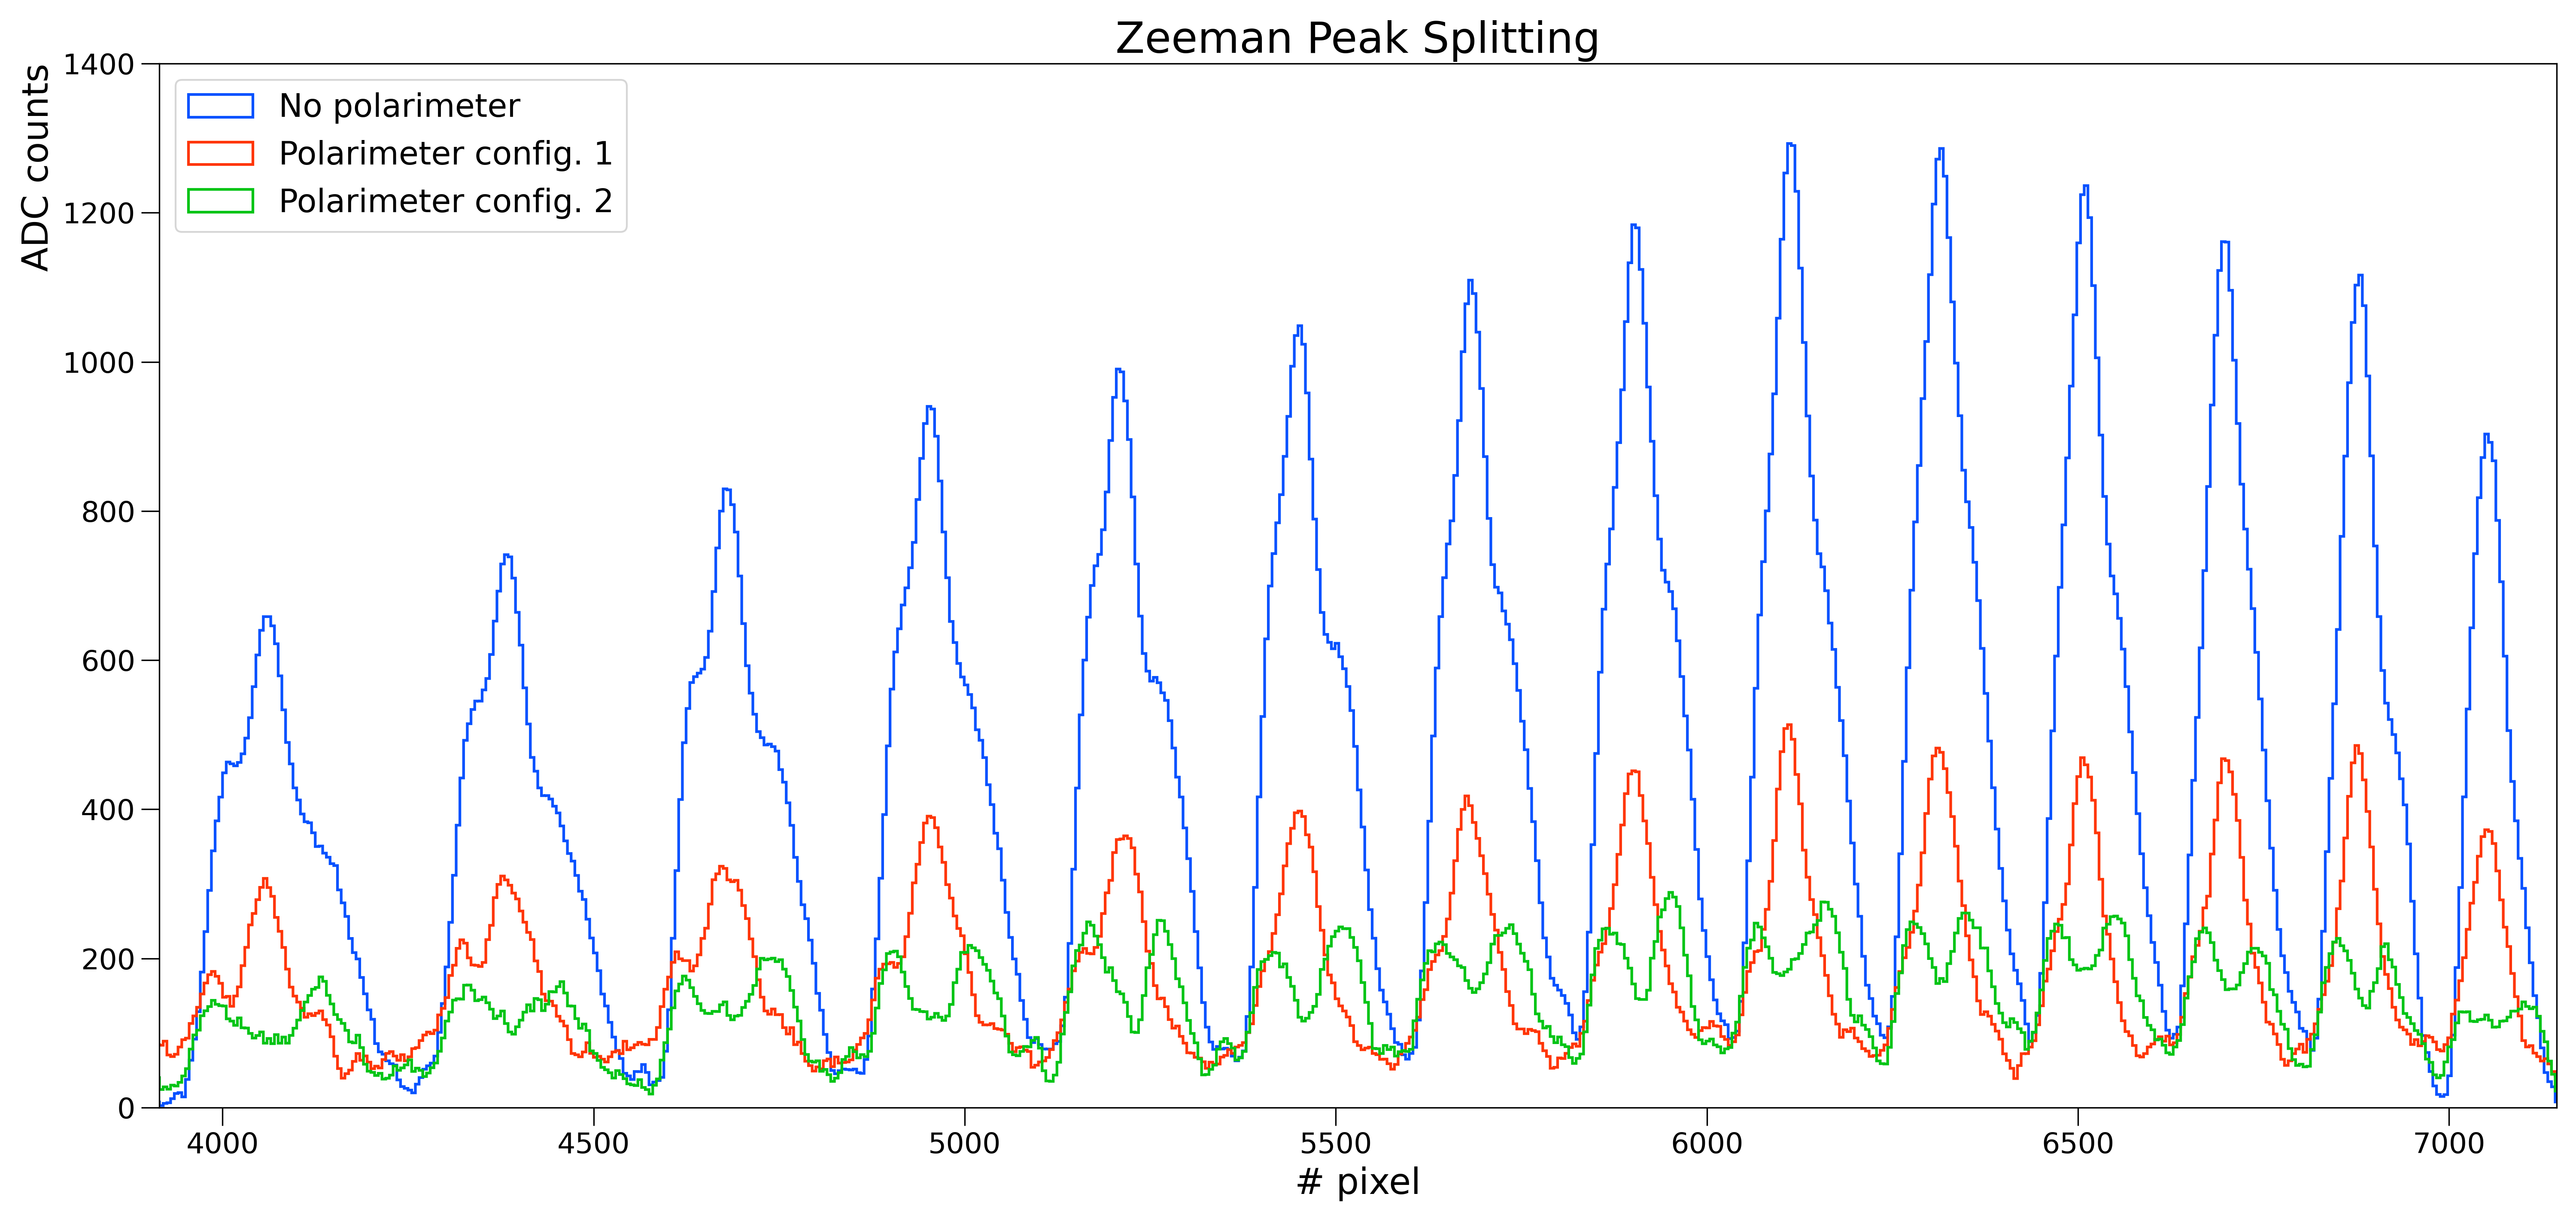
\includegraphics[width=\textwidth]{../Plots/Bon_overlap_big.png}
    \caption{Proiezione sull'asse y dello spettro bidimensionale nelle configurazioni con e senza polarizzatore}
    \label{i:spettro2d_overlap}
\end{figure*}

% \begin{itemize}
%     \item Un po' di fisica più in dettaglio rispetto all'introduzione (polarizzazione ecc) + aspettative "teoriche"
%     (intensità picchi ecc)
%     \item Plot istogrammi sovrapposti 
%     \item Deduzione configurazioni polarimetro dal plot 
% \end{itemize}

Si analizzano i dati acquisiti ruotando il campo magnetico, cioè osservando la radiazione emessa in direzione ortogonale
a $\vec{\text{B}}$. In questo caso, i termini associati a $\Delta \text{m} = 0$ presentano polarizzazione lineare,
mentre quelli relativi a $\Delta \text{m} = \pm 1$ sono polarizzati circolarmente in senso orario o antiorario. Ci si
aspetta quindi di osservare un tripletto, cioè la formazione di tre righe equispaziate visibili nella direzione di
propagazione trasversa al campo. Successivamente, si inserisce un filtro polarizzatore di fronte alla lente condensante,
che viene impiegato in due configurazioni, non note a priori. Se il polarizzatore fa passare prevalentemente la
componente della luce polarizzata parallelamente alla direzione del campo, allora si osserva una sola riga; se invece,
ruotando il filtro, questo fa passare la componente della luce con polarizzazione ortogonale al campo, allora la
transizione centrale viene soppressa e si osservano solamente i due picchi laterali. Conseguentemente ci si aspetta che
l'intensità della radiazione sia significativamente ridotta con l'inserimento del filtro polarizzatore.  
In \autoref{i:spettro2d_overlap} è riportata la proiezione sull'asse y dello spettro bidimensionale, nelle tre
configurazioni precedentamente descritte. Si nota che, in generale, l'apparato non permette di risolvere
sufficientemente bene le transizioni: questo è particolarmente evidente in assenza del filtro, in quanto non è possibile
distinguere i tre picchi di interferenza distinti che ci si aspetterebbe. Inoltre, si osserva che nella prima
configurazione lo spettro è caratterizzato dalla presenza di un unico picco, mentre nella seconda da un doppietto: da
ciò si deduce che nel primo caso il polarizzatore è posto lungo la direzione del campo, mentre nella seconda è ruotato
di 90 gradi. 

\end{document}
